\documentclass[10pt]{article}

\addtolength{\oddsidemargin}{-.875in}
\addtolength{\evensidemargin}{-.875in}
\addtolength{\textwidth}{1.75in}

\addtolength{\topmargin}{-.875in}
\addtolength{\textheight}{1.75in}

\openup 1em

%macro for commenting
\usepackage{color}
\newcommand{\leo}[1]{{\color{blue}{\it leo: #1}}}

% \newcommand{\Xbeta}{ X_i \theta}
\newcommand{\xbeta}{ x_i \beta}
\newcommand{\xtheta}{ x_i \theta}
% \newcommand{\xbetaij}{ x_{ij}^T \theta}
\newcommand{\sgamma}{s_{ij}^T\gamma_i}

\usepackage[round]{natbib}

\usepackage{rotating}
\usepackage{graphicx}
\usepackage{subcaption}

\usepackage{float}


\usepackage{amsthm,amsmath} 
\usepackage{amssymb}
\usepackage{subcaption}

\newtheorem{theorem}{Theorem}
\newtheorem{lemma}{Lemma}
\newtheorem{corollary}{Corollary}
\newtheorem{remark}{Remark}


\usepackage{algorithm}
\usepackage{algpseudocode}

\usepackage{mhequ}
\newcommand{\be}{\begin{equs}}
\newcommand{\ee}{\end{equs}}
\newcommand{\bb}[1]{\mathbb{#1}}
\newcommand{\mc}[1]{\mathcal{#1}}
\DeclareMathOperator{\Binom}{Binomial}
\DeclareMathOperator{\No}{No}
\DeclareMathOperator{\PG}{PG}
\DeclareMathOperator{\IG}{Inverse-Gamma}
\DeclareMathOperator{\Ga}{Gamma}
\DeclareMathOperator{\Bern}{Bernoulli}
\DeclareMathOperator{\U}{Uniform}
\DeclareMathOperator{\Poi}{Poisson}
\DeclareMathOperator{\NB}{NB}
\DeclareMathOperator{\cov}{cov}
\DeclareMathOperator{\var}{var}
\DeclareMathOperator{\diag}{diag}
\DeclareMathOperator{\Diag}{Diag}
\newcommand{\KL}[2]{\textnormal{KL}\left(#1 \parallel #2\right)}

\DeclareMathOperator{\bigO}{\mc O}
\newcommand{\James}[1]{\textcolor{blue}{#1}}


\thispagestyle{empty}
\baselineskip=28pt

\title
{{Calibrated Data Augmentation for Scalable \\ Markov Chain Monte Carlo}}


\author{
     Leo L. Duan,
     James E. Johndrow,
     David B. Dunson
    % \textsuperscript{*}\footnotemark[2]\and
}

 
\begin{document}
    
\maketitle

{\bf Abstract:} Data augmentation is a common technique for building tuning-free Markov chain Monte Carlo algorithms. Although these algorithms are very popular, 
autocorrelations are often high in large samples, leading to poor computational efficiency.  This phenomenon has been attributed to a discrepancy between Gibbs step sizes and the rate of posterior concentration.  In this article, we propose a family of calibrated data augmentation algorithms, which adjust for this discrepancy by inflating step sizes.  A Metropolis-Hastings step is included to account for the slight discrepancy between the stationary distribution of the resulting sampler and the exact posterior distribution.  The approach is applicable to a broad variety of existing data augmentation algorithms, and we focus on three popular models: probit, logistic and Poisson log-linear.  Theoretical support is provided and dramatic gains are shown in applications.
\vskip 12pt

%\baselineskip=12pt
%\par\vfill\noindent
{\noindent  KEY WORDS:  Bayesian probit; Bayesian logit; Big $n$; Data Augmentation; Maximal Correlation; Polya-Gamma.}
%\par\medskip\noindent
%\clearpage\pagebreak\newpage
\pagenumbering{arabic}

\section{Introduction}

With the deluge of data in many modern application areas, there is pressing need for scalable computational algorithms for inference from such data, including uncertainty quantification (UQ).  Somewhat surprisingly, even as the volume of data increases, uncertainty often remains sizable.  Examples in which this phenomenon occurs include financial fraud detection \citep{ngai2011application}, disease mapping \citep{wakefield2007disease} and online click-through tracking \citep{wang2010click}.  Bayesian approaches provide a useful paradigm for quantifying uncertainty in inferences and predictions in these and other settings.

The standard approach to Bayesian posterior computation is Markov chain Monte Carlo (MCMC) and related sampling algorithms. Non-sampling alternatives, such as variational Bayes, tend lack general accuracy guarantees. However, it is well known that conventional MCMC algorithms often scale poorly in problem size and complexity. Due to its sequential nature, the computational cost of MCMC is the product of two factors: the evaluation cost at each sampling iteration and the total number of iterations needed to obtain an acceptably low Monte Carlo error. The latter is related to the properties of the Markov transition kernel; we will refer to this informally as the \emph{mixing properties} of the Markov chain. 

In recent years, a substantial literature has developed focusing on decreasing computational cost per iteration (\cite{minsker2014robust,srivastava2015wasp,conrad2015accelerating} among others), mainly through accelerating or parallelizing the sampling procedures at each iteration. Moreover, myriad strategies for improving mixing have been described in the literature. For Metropolis-Hastings (M-H) algorithms, improving mixing is usually a matter of contructing a better proposal distribution. An important difference between M-H and Gibbs is that one has direct control over step sizes in M-H through choice of the proposal, while Gibbs step sizes are generally not tunable; on the other hand, finding a good proposal for multi-dimensional parameters in M-H is significantly more challenging compared to Gibbs sampling. Thus, improving mixing for Gibbs has historically focused on decreasing autocorrelation by changing the update rule itself, for example by parameter expansion (PX), marginalization, or slice sampling.\footnote{Although strictly speaking, slice sampling is just an alternative approach to sampling from a full conditional distribution, in practice, it is often an alternative to data augmentation, so that using a slice sampling strategy results in the removal of a data augmentation step from an alternative Gibbs sampler.} 

The theory literature on behavior of MCMC for large $n$ and/or $p$ is arguably somewhat limited. Many authors have focused on studying mixing properties by showing 
an ergodicity condition, such as geometric ergodicity \citep{roberts2004general,meyn2012markov}. This generally yields bounds on the convergence rate and spectral gap of the Markov chain, but \cite{rajaratnam2015mcmc} observe that in many cases, these bounds converge to one exponentially fast in $p$ or $n$, so that no meaningful guarantee of performance for large problem sizes is provided by most existing bounds. In the probability literature, a series of papers have developed an analogue of Harris' theorem and ergodic theory for infinite-dimensional state spaces \citep{hairer2011asymptotic}. Recent work verifies the existence of MCMC algorithms for computation in differential equation models with dimension-independent spectral gap \citep{hairer2014spectral}. In this example, the algorithm under consideration is an M-H algorithm, and it is clear that the proposal must be tuned very carefully to achieve dimension independence. Other work has studied the properties of the limiting differential equation that describes infinite-dimensional dynamics of MCMC.

A recent paper (\cite{johndrow2016inefficiency}) studies popular data augmentation algorithms for posterior computation in probit \citep{albert1993bayesian} and logistic  \citep{polson2013bayesian} models, showing that the algorithms fail to mix in large sample sizes when the data are imbalanced. An important insight is that the performance can be largely explained by a discrepancy between the rate at which Gibbs step sizes and the width of the high-probability region of the posterior converge to zero as the sample size increases. Thus, since Gibbs step sizes are generally not tunable, slow mixing is likely to occur as the sample size grows unless the order of the step size happens to match the order of the posterior width. This implies that if a way to directly control the step sizes of the Gibbs sampler could be devised, it would be possible to make the mixing properties of the sampler insensitive to sample size by scaling the step sizes appropriately. This is similar to the conclusion of \cite{hairer2014spectral}, except in this case, we have growing $n$ instead of growing $p$.

In this article, we propose a method for tuning step sizes by introducing auxiliary parameters that change the variance of full conditional distributions for one or more parameters. As these ``calibrated'' data augmentation algorithms alter the invariant measure, one can use the Gibbs step as a highly efficient M-H proposal, thereby recovering the correct invariant, or view the resulting algorithm as a perturbation of the original Markov chain.  In this article, we focus on the former strategy, providing theoretical support and showing very substantial practical gains in computational efficiency attributed to our calibration approach.

\section{Calibrated Data Augmentation}
Data augmentation Gibbs samplers alternate between sampling  latent data $z$ from their conditional posterior distribution given model parameters $\theta$ and observed data $y$, and sampling parameters $\theta$ given $z$ and $y$; either of these steps can be further broken down into a series of full conditional sampling steps but we focus for simplicity on algorithms of the form \citep{tanner1987calculation}: 
\be \label{eq:da}
z \mid \theta, y &\sim h(z; m(\theta),y) \\
\theta \mid z,y &\sim f(\theta; \mu, \Sigma),
\ee
where $f$ belongs to a location-scale family, such as the Gaussian, with $\mu$ as its conditional location and $\Sigma$ its conditional scale; $h$ is also a distribution that can be sampled directly. We use $\pi(.)$ to denote the density.
Letting $i=1,\ldots,n$ index the samples, with $y=(y_1,\ldots,y_n)$, often $\pi(z \mid \theta,y) = 
\prod_{i=1}^n \pi(z_i; m_i(\theta), y_i)$, so that the latent data for different subjects can be sampled independently.  Popular data augmentation algorithms independently sample the $z_i$'s and then draw $\theta$ simultaneously (or at least in blocks) from a multivariate Gaussian or other standard distribution.  Data augmentation algorithms are particularly common for generalized linear models (GLMs), with $\bb E(y_i \mid x_i, \theta) = g^{-1}(x_i \theta)$ and a conditionally Gaussian prior distribution chosen for $\theta$. We focus in particular on binomial probit, binomial logistic, and Poisson log-linear as motivating examples.

Particularly as $n$ increases, a key problem can arise in implementing update rule \eqref{eq:da}; in particular, the step size of $\var(\theta_t \mid \theta_{t-1})$ from the $(t-1)$th iteration to the $t$th iteration can be substantially smaller than the posterior $\var(\theta \mid y)$.  This leads to slow mixing.  To solve this problem, we replace these sampling steps with two steps from a {\it calibrated} data augmentation (CDA); since the target is modified because of the calibration, we use an M-H step to preserve the original target. 

We first present the general algorithm, then use examples to illustrate the details.

 \subsection{General Algorithm}
 
%  We assume the parameters are multi-dimensional and can be divided into two groups $\{ \theta, \tau\}$, with $\theta$ and $\tau$ sampled separately based on their conditional posterior distributions and $\theta$  susceptible to slow mixing.  For notational ease, we focus on $\theta$ and omit the conditioning on $\tau$ in the rest of the section.  
 
The key problem with algorithm \eqref{eq:da} is that the step size being too small compared to $\var(\theta \mid y)$. Since $\var(\theta_{t} \mid \theta_{t-1}) \ge \bb E_{z\mid \theta_{t-1} } \var(\theta_{t} \mid z,y) $, we propose to increase the expected conditional variance $\bb E_{z\mid \theta_{t-1} } \var(\theta_{t} \mid z,y) $  to adjust the step size and match the marginal variance $\var(\theta \mid y)$. Through this, each sampling iteration from conditional posterior could explore the marginal posterior region efficiently. For simpler notation, we write the expected conditional variance as $\bb E_{z} \var(\theta \mid z,y) $.

To start the calibration, note the two steps in \eqref{eq:da} are associated with two equivalent factorizations of likelihood $L(\theta;y)$ with augmented data $z$:

 \be \label{eq:da_decomposition}
 L(\theta;y)= \int \pi\left( z \mid \theta,y \right)\pi( \theta \mid y) d z  =  \int \pi\left(\theta \mid z,y \right)\pi(z \mid y) d z .
 \ee

Depending on the form of $\mbox{var } (\theta \mid z,y)$ in the second step, there are two different ways to induce an increase in $\bb E_z \text{var}(\theta \mid z, y)$. If $\mbox{var } (\theta \mid z,y)$ is free from $z$ (hence $\bb E_z \text{var}(\theta \mid z, y) = \mbox{var } (\theta \mid z,y)$), we directly modify it via changing $\pi\left(\theta \mid z,y \right)$ in the second factorization of \eqref{eq:da_decomposition}; if $\mbox{var } (\theta \mid z,y)$ is a function of $z$, we modify the first step by changing $\pi\left( z \mid \theta,y \right)$ in the first factorization of \eqref{eq:da_decomposition}, in order to stochastically influence the value of $z$ and $\mathbb{E}_z \mbox{var } (\theta \mid z,y)$.

By ``change'', we meant a {\it relaxation} of a fixed distribution parameter to a tunable working parameter $r$. Therefore, this minor change does not impact the posterior distribution families $h$ and $f$ in \eqref{eq:da}, nor the integrability for obtaining the marginal likelihood via \eqref{eq:da_decomposition}. The two adjustment approaches will be concretely illustrated via examples in the next few subsections.

As the change alters the target distribution, we use an M-H step to correct the difference. As the modification in variance usually impacts the location parameter of $\theta$ as well, to facilitate higher M-H acceptance rate, we introduce another auxiliary parameter $b$ to allow further adjusting of the location parameter of $\theta$.

The CDA sampling algorithm involves generating a new proposal $\theta^*$ via two steps:
 
  \be
 z  \mid \theta, y& \sim h_{r,b}(z; m(\theta), y) \\
 \theta^*  \mid z, y&\sim f( \theta^*|\mu(r, b),\Sigma(r))
 \ee
 and accepting the proposal $ \theta^*$ with probability (with its derivation deferred to the theory section):
 \be
 1 \wedge  \frac{L(\theta^*; y) L_{r,b}(\theta ; y)} {L(\theta; y) L_{r,b}(\theta^*; y)},
 \ee
where $L_{r,b}(\theta ; y)$ is the integrated marginal likelihood after inclusion of $r$ and $b$:
 \be \label{eq:cda_decomposition}
 L_{r,b}(\theta ; y) = \int \pi_{r,b}\left( z \mid \theta,y \right)\pi_{r,b}( \theta \mid y) d z.
  \ee

There are three important properties about CDA. First, for any fixed $(r,b)$ in suitable domain, $L_{r,b}(\theta ; y)$ is a proper likelihood function, because the calibration does not alter the families of distribution in \eqref{eq:da_decomposition}. Second, a constrained domain $\mc R$  can be specified for $r$ so that the step size is always greater or equal to the un-calibrated one. Third,  $L(\theta;y)$ is a special case of  $L_{r,b}(\theta ; y)$ for certain $r$ and $b$ (e.g. mostly $L(\theta;y)=L_{1,0}(\theta;y)$). When that happens, M-H step will always accept the proposal with probability $1$ and the algorithm reverts to Gibbs sampling. Therefore, CDA sampling is a generalized algorithm of Gibbs sampling for data augmentation.



\subsection{Initial example: probit with intercept only}

We first use a simple model to illustrate the calibration procedure for one parameter and demonstrate the effects of step size on mixing. Consider a probit model with intercept only

\be
y_i \sim \Bern(p_i), \quad p_i = \Phi(\theta) \quad i=1,\ldots,n,\quad \pi(\theta) \propto 1,
\ee
where $\Phi(\theta)$ is the cumulative distribution function of standard normal; $\pi(\theta)$ is the flat prior for $\theta$. The basic data augmentation algorithm \citep{albert1993bayesian} has the update rule
\be
z_i \mid \theta, y_i &\sim \left\{ \begin{array}{cc} \No_{[0,\infty)}( \theta,1) & \text{ if } y_i = 1 \\ \No_{(-\infty,0]}( \theta,1) & \text{ if } y_i = 0 \end{array} \right.  \quad i=1,\ldots,n\\
\theta \mid z, y &\sim \No( \sum_i z_i /n, 1/n ),
\ee
where $\No_{[a,b]}(\mu,\sigma^2)$ is the normal distribution with mean $\mu$ and variance $\sigma^2$ truncated to the interval $[a,b]$. \cite{johndrow2016inefficiency} show that when $\sum_i y_i$ is fixed and much smaller than $n$, $\var(\theta_t \mid \theta_{t-1})$ is approximately $n^{-1} \log n$, while the width of the high probability density region of the posterior is of order $(\log n)^{-1}$. The rate difference causes critical mixing issue in rare event modeling.

As the conditional variance $\mbox{var}(\theta\mid z,y)$ is free from $z$, we replace the fixed small variance $1/n$ with a tunable scalar $r/n$ and adjust the location with another scalar parameter $b$. We further require $r\ge 1$ to ensure step size is unchanged or increased. Utilizing the equivalent factorizations in \eqref{eq:da_decomposition}, this is the same as changing the scale of $z_i \mid\theta,y_i$ from $1$ to $r$ and the mean from $\theta$ to $\theta+b$. These adjustments lead to a new sampling algorithm with proposal $\theta^*$:

\be \label{eq:cda-probit-intercept}
z_i \mid \theta, y_i &\sim \left\{ \begin{array}{cc} \No_{[0,\infty)}( \theta+b,r) & \text{ if } y_i = 1 \\ \No_{(-\infty,0]}( \theta+b,r) & \text{ if } y_i = 0 \end{array} \right. \quad i=1,\ldots,n \\
\theta^* \mid z,y &\sim \No(  \sum_i(z_i-b)/n, r/n),
\ee
and accepting $\theta^*$ with probability

\be
1 \wedge  \prod_i  \frac{ L_{r,b}(\theta;y_i) L(\theta^*;y_i)}{ L_{r,b}(\theta^*;y_i)L(\theta;y_i) },
\label{eq:mh-criterion-probit-intercept}
\ee
where $L_{r,b}(\theta;y_i) =  \Phi\big( \frac{\theta+b}{\sqrt{r}}\big) ^{y_i} \Phi \big( -\frac{\theta+b}{\sqrt{r}}\big) ^{(1-y_i)}$ and $L(\theta;y_i)  = L_{1,0}(\theta;y_i)$. This calibration increases the step size of the proposal to $\var(\theta^* \mid \theta_{t-1}) \ge \bb E_{z}\var(\theta^* \mid z)   = r/n$. To match to the approximate width of marginal high probability density region $(\log n)^{-1}$, theoretically we need $r \approx n/\log n$.


To illustrate, we set $\sum_i y_i =1$ and $n=10^4$, and run the new algortihm for these data with different values of $r$ ranging from $r=1$ to $r=5,000$, among which $r=1,000 \approx n/\log n$ corresponding to the theoretically optimal value. In this simple example, it is easy to compute a ``good'' value of $b = -3.7 (\sqrt r -1)$, as it results in $\mbox{pr}(y_i = 1) = \Phi(-3.7) = n^{-1}\sum_i y_i  \approx 10^{-4}$ in the proposal distribution. This choice ensures that each $L_{r,b}(\theta;y_i) $ for different $r$ are centered around the center of $L(\theta;y_i)$, so that the proposal is around the high posterior density of the target, so that it has high acceptance rate.

Figure~\ref{probit_demo_intercept_proposal} plots autocorrelation functions (ACFs) for these different samplers. Autocorrelation is very high even at lag 40 for $r=1$ (which corresponds to the basic Gibbs sampler), while increasing $r$ leads to dramatic improvements in mixing. There are no further gains in increasing $r$ from the theoretically optimal value of $r=1,000$ to $r=5,000$. Figure~\ref{probit_demo_intercept_density} shows the density estimates under $L_{r,b}(\theta;y)$; they are all centered about the same values due to the adjustment of $b$, and with variance increasing according to $r$.  With M-H adjustment the differences are removed; the M-H step has average acceptance rate close to 1 for $r=10$ and $100$, 0.6 for $r=1,000$, and 0.2 for $r=5,000$.

\begin{figure}[H]
 % \centering
  \begin{subfigure}[b]{0.45\textwidth}
 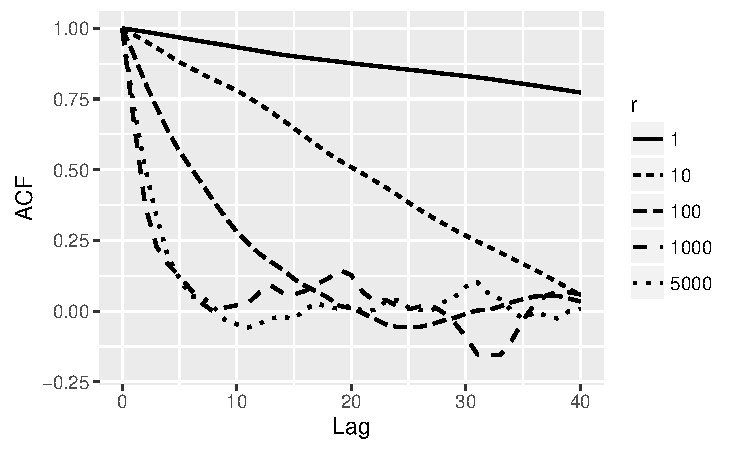
\includegraphics[width=1\textwidth]{probit_demo_acf.pdf}
  \caption{ACF for CDA with different r controlling the step size.}
 \label{probit_demo_intercept_proposal}
\end{subfigure}
  \hfill
    \begin{subfigure}[b]{0.45\textwidth}
 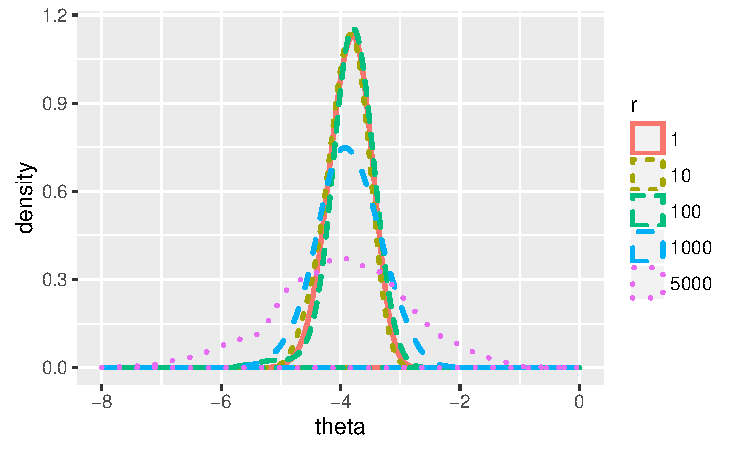
\includegraphics[width=1\textwidth]{density_probit.pdf}
  \caption{Density estimates of the integrated marginal $L_{r,b}$ with different r.}
   \label{probit_demo_intercept_density}
\end{subfigure}
  \caption{ Autocorrelation functions (ACFs) and density estimates for $L_{r,b}$ in intercept-only probit model.}
 \label{probit_demo_intercept}
 \end{figure}

\subsection{Probit regression example}

The intercept only probit model illustrates the adjustment of variance when $\theta$ is a single parameter. When $\theta$ is multi-dimensional, the calibration needs to be applied on the matrix of conditional covariance. To illustrate this scenario, we consider a probit regression with flat prior:

\be
y_i \sim \Bern(p_i), \quad p_i = \Phi(x_i \theta) \quad i=1,\ldots,n, \quad \pi(\theta) \propto 1
\ee
and Gibbs sampling rule \citep{albert1993bayesian}:
\be
z_i \mid \theta, x_i, y_i &\sim \left\{ \begin{array}{cc} \No_{[0,\infty)}(x_i \theta,1) & \text{ if } y_i = 1 \\ \No_{(-\infty,0]}(x_i \theta,1) & \text{ if } y_i = 0 \end{array} \right. \quad i=1,\ldots,n \\
\theta \mid z, x, y &\sim \No((X'X)^{-1} X'z, (X'X)^{-1}),
\ee
where $X= \{x'_1,\ldots, x'_n\}'$ is the predictor matrix.

 Similar to the intercept only model, we can directly modify the $\mbox{var}( \theta | z,y)$ as it is free from $z$. we begin calibration by changing the variance of $z_i$ from $1$ to a parameter $r_i$; we add $b_i$ to the predictor $\xtheta$ to allow optimizing for M-H acceptance rate. This yields new update rule of sampling proposal from:
 
 \be \label{eq:cda-probit}
z_i \mid \theta, x_i, y_i &\sim \left\{ \begin{array}{cc} \No_{[0,\infty)}(x_i \theta+b_i,r_i) & \text{ if } y_i = 1 \\ \No_{(-\infty,0]}(x_i \theta+b_i,r_i) & \text{ if } y_i = 0 \end{array} \right. \quad i=1,\ldots,n \\
\theta^* \mid z, X &\sim \No\big((X'R^{-1}X)^{-1} X'R^{-1}(z-b), (X'R^{-1}X)^{-1} \big),
\ee
with $R = \diag(r_1,\ldots,r_n)$, $b= \{b_1,\ldots,b_n\}'$, and accepting $\theta^*$ with probability:
\be
1 \wedge  \prod_i  \frac{L_{r,b}(\xtheta;y_i) L(\xtheta^*;y_i)}{  L_{r,b}(\xtheta^*;y_i)L(\xtheta;y_i) },
\label{eq:mh-criterion}
\ee
where  $L_{r,b}(\xtheta;y_i) = \Phi\big( \frac{\xtheta+b_i}{\sqrt{r}}\big) ^{y_i} \Phi \big( -\frac{\xtheta+b_i}{\sqrt{r}}\big) ^{(1-y_i)}$ and $L(\xtheta;y_i)  = L_{1,0}(\xtheta;y_i) $.

The calibration generates an adjustable covariance matrix $\mbox{var}(\theta^* \mid z, X) = (X'R^{-1}X)^{-1}$. We allow $r$ and $b$ to vary over index $i$ so that the covariance can be flexibly tuned. In general, we can tune the covariance to be approximately close to the marginal covariance $\mbox{var}(\theta \mid y)$, so that the sampler can explore the high posterior density region efficiently. We also require all $r_i\ge 1$ so that the variance can only increase.

We will continue discussing the choice for $r$ and $b$ in section \ref{parameter_adapation}, after demonstrating the second calibration strategy when  $\mbox{var}( \theta | z,y)$ is not free from $z$.

\subsection{Logistic regression example}

The probit examples illustrate the scenario when  $\mbox{var}( \theta | z,y)$ is free from $z$, the step size can be directly calibrated through changing the second step of \eqref{eq:da}. When $\mbox{var}( \theta | z,y)$  does involve $z$, the calibration can be achieved by changing the first step of \eqref{eq:da}. We now demonstrate this approach. 

Consider the logistic regression model with flat prior:
\be
y_i \sim \Bern(p_i), \quad p_i = \frac{\exp(x_i \theta)}{1+\exp(x_i \theta)} \quad i=1,\ldots,n, \quad \pi(\theta) \propto 1
\ee
and a two-step update rule based on Polya-Gamma data augmentation \citep{polson2013bayesian}:
 \be
 z_i \mid \theta, x_i &\sim {\PG}(1, |\xtheta|) \quad i=1,\ldots,n,\\
\theta \mid z, X, y&\sim \No \left(  (X' Z X)^{-1}   X'  (y-0.5)  ,  (X' Z X)^{-1}  \right),
\ee
where $Z= \diag(z_1,\ldots,z_n)$ and $\PG$ is the Polya-Gamma distribution.

Since $Z$ is random, it would be difficult to directly modify $(X' Z X)^{-1}$ in the second step. Instead, we can stochastically influence the value of $Z$ by modifying the first step. This is achieved by replacing the first Polya-Gamma parameter $1$ with a tunable $r_i$. We require $r_i \in (0,1]$ to ensure step size is unchanged or increased. Intuitively, smaller $r_i$ tends to produce smaller $z_i$ hence larger $z_i^{-1}$ since $\bb{E}z_i= \frac{r_i}{2 a}\tanh(\frac{a}{2})$ for $z_i \sim \PG(r_i, a)$. More rigorously, its first negative moment can be computed as $\bb{E}z_i^{-1}= \int_0^{\infty} \prod_{k=1}^{\infty} (1+ d_k^{-1} t) ^{-r_i} dt$ with $d_k=2(k-\frac{1}{2})^2\pi^2 + \frac{a^2}{2}$ (combining \cite{cressie1981moment} and \cite{polson2013bayesian}). Therefore, smaller $r_i$'s lead to larger expected conditional variance $\bb E_z (X' Z X)^{-1}$.

Similar to the probit example, we add the location adjusting parameter $b_i$ to the linear predictor $x_i\theta$ and allow optimizing for better acceptance rate. The new algorithm is sampling from proposal:
\be
 z_i  \mid \theta, x_i &\sim {\PG}(r_i, |\xtheta+b_i|) \quad i=1,\ldots,n,\\
\theta^*  \mid z, X, y &\sim \No \left(  (X' Z X)^{-1}  X'  (y -r/2- Zb) ,  (X' Z X)^{-1}  \right),
\ee
with acceptance probability:
\be
1 \wedge \prod_i  \frac{  L_{r,b}(\xtheta;y_i) L(\xtheta^*;y_i)}{  L_{r,b}(\xtheta^*;y_i)L(\xtheta;y_i) },
\ee
where 
\be
L_{r,b}(\xtheta;y_i) = & \int_{0}^{\infty}  \exp\{ (\xtheta+b_i) (y_i-r_i/2)\} \exp\bigg\{ -\frac{z_i (\xtheta+b_i)^2}{2}\bigg\} \PG(z_i \mid r_i,0) dz_i \\
= &  \frac{\exp \{ (x_i \theta + b_i)y_i \}}{\{1+\exp(\xtheta +b_i)\}^{r_i}}
\label{eq:prop-marginal-logit}
\ee
and $L(\xtheta;y_i) = L_{1,0}(\xtheta;y_i)$.

\subsection{Choice of calibration parameters}
\label{parameter_adapation}

We now illustrate a simple and efficient strategy for selecting calibration parameters $r=(r_1,\ldots,r_n)$ and $b=(b_1,\ldots,b_n)$, and use them for calibrating the above probit and logistic regression examples. Unlike the intercept probit example, in general it is difficult to analytically calculate the marginal or expected conditional variances. Therefore, we now propose an empirical approach to estimate the difference between the two. Despite being empirical, this method follows the guarantee that the mixing will be accelerated, since the tuned $r$ is constrained in region $\mc R$ where step size can only increase.

For the marginal variance, we use inverse Fisher information for approximation. In large samples, the inverse of Fisher information evaluated at the ``true value'' $\theta_0$ of the parameter is an asymptotic approximation to the posterior marginal covariance. When the expectation of conditional variance is intractable, we can consider the inverse of expected conditional precision as an approximate. Depending on which is convenient to compute, it is useful to choose $r\in \mc R$ to minimize the one of the distances below, :
 
\be
\Delta_{\mc I^{-1}}(\theta_0) &= \|  c_0 \mc  I^{-1}(\theta_0)- \bb E_{z \mid \theta, r, b} \var(\theta^* \mid z)\bigg| \theta_0 \|_F \\
\Delta_{\mc I}(\theta_0) &= \|  \mc  I(\theta_0) / c_0 -   \bb E_{z \mid \theta, r, b} \big(\bb\var(\theta^* \mid z)\big)^{-1} \bigg| \theta_0\|_F
\ee
where $ \mc  I(\theta_0)  = E_y \left[ \left( \frac{\partial}{\partial \theta} \log L(y;\theta) \right)^2 \right]\bigg| \theta_0 $ with expectation taken over the distribution of the data $y$ under the target likelihood $L$, and $\| A \|_F$ is the Frobenius norm of $A$; $\bb E_{z \mid \theta, r, b}$ is taken with respect to the latent variable $z \mid \theta$ under $L_{r,b}(\theta; y)$. By default, we set $c_0=1$. The parameter $c_0$ is a scalar constant reserved for adjusting when this approximating approach over-estimated the needed step size. When that happens, it is shown by a very low acceptance rate, as the calibrated step size is too wide and most of proposals fall out of the high posterior region of $L$; it would then be useful to use smaller $c_0$ to reduce the step size.


Since there is no fixed $\theta_0$ in Bayesian paradigm, we use the empirical maximum-a-posteriori (MAP) estimate $\hat \theta_{t}= \underset{\theta\in \{ \theta_1, \ldots, \theta_t\}}{\arg\max } L (\theta ; y) \Pi^0(\theta)$, based on posterior samples $\{ \theta_1, \ldots, \theta_t\}$ collected in the first $t$ iterations, and $ \Pi^0(\theta)$ is the prior. We then dynamically update $r_t,b_t$ based on $\hat \theta_{t}$. Specifically, we choose $r_{t+1}$ to minimize $\Delta_{\mc I^{-1}}(\hat \theta_t)$ or $\Delta_{\mc I}(\hat \theta_t)$, and set $b_{t+1}$ to minimize the difference between $L_{1,0}(\hat \theta_t;y)$ and $L_{r_{t+1},b_{t+1}}(\hat \theta_t;y)$. Thus, we use $r$ to adjust the expected conditional variance based on $L_{r,b}$ to match the marginal variance based on $L$; and we use $b$ to make $L_{r,b}$ close to $L_{1,0}$ in the neighborhood of $\hat \theta_t$. Intuitively, this will make the proposal distribution closer to the target, and correspondingly increase the M-H acceptance rate.

The proposal kernel we describe above is \emph{adaptive}; that is, we have a collection of proposal kernels $\mc Q = \{Q_{r,b}\}_{(r,b) \in \bb \mc R \times \mc B}$, and we choose a different member of $\mc Q$ to create the proposal when $\hat \theta_{t}$ is changed. For every $Q_{r,b}$, the \emph{target}  $\Pi$ for the resulting transition kernel is the same as the original Gibbs sampler,  because of the Metropolis-Hastings rejection step.  In general, ergodicity of adaptive algorithms requires a diminishing adaptation condition; a general condition of this sort is given in \cite{roberts2007coupling}. Although the algorithm we describe is unlikely to satisfy diminishing adaptation, the condition is trivially satisfied by any algorithm that stops adaptation after a fixed number of iterations. Thus, for simplicity, we choose a tuning period length, after which we fix $r,b$ at their current values. More sophisticated adaptation schemes could be devised; however, the fixed tuning period works well empirically.


For a concrete illustration, we now return to the example of the probit regression. Letting $\hat\eta_i = x_i \hat\theta_t$ denote the linear predictor corresponding to the empirical MAP, during the tuning period, the marginal approximate and the expected conditional variance are:
\be
c_0 \mc I^{-1}(\hat\theta_t) &= c_0 ( X'\diag\bigg\{\frac{\phi(\hat\eta_i)^2}{ {\Phi(\hat\eta_i)(1- \Phi(\hat\eta_i))}}\bigg\} _{i=1,\ldots n} X)^{-1},\qquad \bb E_{z \mid \theta, r, b}  \var (\theta^* \mid z) = (X' R^{-1} X)^{-1}
\ee
respectively, where $\phi$ is the standard normal density. Therefore, we set $r_i = \hat r_i \vee 1$ with $\hat r_i= c_0 \frac{\Phi(\hat\eta_i)(1- \Phi(\hat\eta_i))} {\phi(\hat\eta_i)^2}$, as $\Delta_{\mc I^{-1}}(\hat\theta_t)=0$ if all $\hat r_i \ge 1$.  The $r_i$'s can be calculated using this expression at low cost without calculating the full information matrix. We set $b_i = \hat\eta_i (\sqrt{r_i}-1)$ to ensure that $|L_{r,b}(\hat\eta_i;y_i) - L(\hat\eta_i;y_i)|=0$.

To illustrate, we use a probit regression with an intercept $x_{i,0}=1$ and two predictors $x_{i,1},x_{i,2}\sim \No(1,1)$, with ``true'' $\theta=(-5,1,-1)'$, generating $\sum y_i=20$ among $n=10,000$. The \cite{albert1993bayesian} DA algorithm mixes slowly (Figure~\ref{probit_reg_trace} and \ref{probit_reg_acf}). 
 We also consider the parameter expansion algorithm (PX-DA) \citep{liu1999parameter,meng1999seeking}, which re-parameterizes $\theta$ with a redundant scale parameter. The key difference is that PX-DA does not increase the conditional variance of $\theta$ and the extra parameter is very constrained as $\theta$-marginal likelihood needs to be unaltered, therefore it cannot directly solve the small step size problem. As the result, PX-DA only mildly reduces the correlation. Using CDA, we initially tuned $r$ and $b$ for $100$ steps using the Fisher information at default $c_0=1$, and collected samples afterwards with fixed $r$ and $b$. We obtain dramatically better mixing at an average acceptance rate of $0.6$.

 
\begin{figure}[H]
 % \centering
  \begin{subfigure}[b]{0.45\textwidth}
 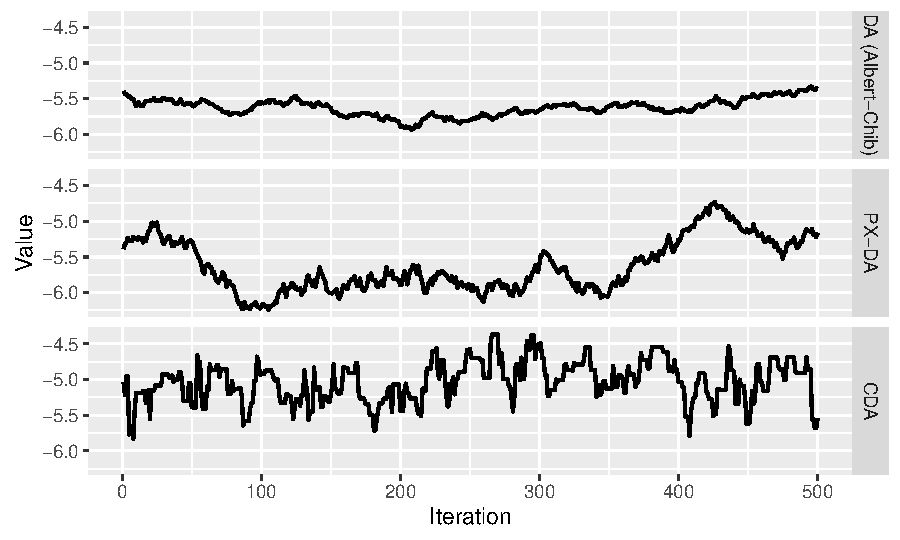
\includegraphics[width=1\textwidth]{probit15_trace_plot.pdf}
  \caption{Traceplot for the original DA, parameter expanded DA and CDA algorithms.}
  \label{probit_reg_trace}
\end{subfigure}
  \hfill
   \begin{subfigure}[b]{0.45\textwidth}
 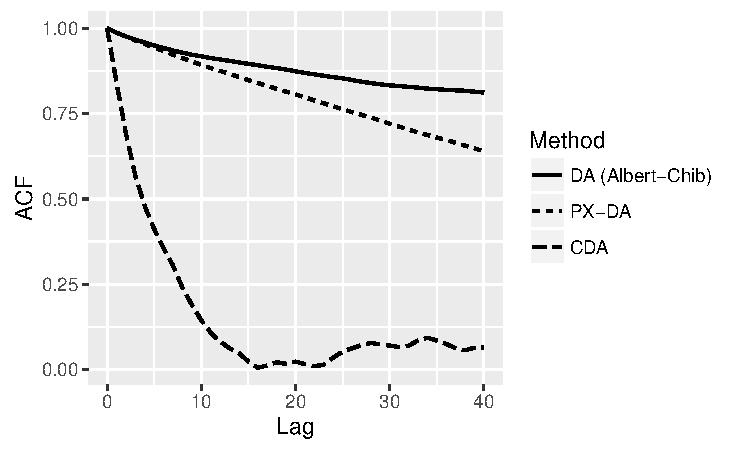
\includegraphics[width=1\textwidth]{probit15_acf.pdf}
  \caption{ACF for original DA, parameter expanded DA and CDA algorithms.}
    \label{probit_reg_acf}
\end{subfigure}
 \caption{Panel (a) demonstrates in traceplot and panel (b) in autocorrelation the substantial improvement in CDA by correcting the variance mis-match in probit regression with rare event data, compared with the original \citep{albert1993bayesian} and parameter-expanded methods \citep{liu1999parameter}.}
 \end{figure}
 
 
 As for the second example of the logistic regression, since $\bb E z$ is more convenient to compute than $\bb E z^{-1}$ , we minimize the distance $\Delta_{\mc I}(\hat\theta_t)$ based on precision matrices. Letting $\hat\eta_i = x_i \hat\theta_t$ based on empirical MAP during tuning, the marginal approximate and the conditional precision matrices are:

 \be
 \mc I(\hat \theta_t)/c_0 &= ( X' \diag\bigg\{\frac{\exp(\hat\eta_i)}{ \{1+\exp(\hat\eta_i)\} ^2}\bigg\}_{i=1,\ldots ,n} X)/c_0, \\
  \bb  E_{z \mid \theta, r, b}  \big (\var (\theta^* \mid z) \big)^{-1} \bigg| \hat\theta_t &=  X'  \diag\bigg\{ \frac{r_i}{2 |\hat\eta_i+b_i|}\tanh\Big(\frac{|\hat\eta_i+b_i|}{2} \Big)\bigg\}_{i=1,\ldots ,n} X
\ee

We set $r_i=\hat r_i \wedge 1$ with $\hat r_i= \frac{1}{c_0}\frac{\exp(\hat\eta_i )}{ \{1+\exp(\hat\eta_i )\} ^2} {2 |\hat\eta_i +b_i|}/ \tanh(\frac{|\hat\eta_i +b_i|}{2})$, as $\Delta_{\mc I}(\hat\theta_t)=0$ if all $\hat r_i \le1$ ; comparing $L_{r,b}(\theta \mid y )$ and $L(\theta \mid y )$, we set $b_i = \log[  \{1+\exp(\hat\eta_i)\}^{1/r_i} -1] - \hat\eta_i$ to minimize the difference.

To illustrate, we use a two parameter intercept-slope model with $x_{i,0}=1$,  $x_{i,1}\sim \No(0,1)$ for $i=1,\ldots, n$ and ``true'' $\theta=(-9,1)'$. With $n= 10^5$, we obtain rare event data with  $\sum y_{i} = 50 $.  Shown in Figure~\ref{logit_random_mixing}, the original DA algorithm  \citep{polson2013bayesian} mixes slowly. We consider a simpler M-H algorithm with multivariate normal proposal with inverse Fisher information as the covariance (denoted as MH-MVN). Since the normal proposal and the logistic target are in different distribution families, the mixing does not get significantly improved. For CDA we tuned $r$ and $b$ for $100$ steps using the Fisher information at default $c_0=1$, reaching an acceptance rate of $0.8$, then collected samples. CDA has dramatically better mixing.




\begin{figure}[H]
 % \centering
  \begin{subfigure}[b]{0.49\textwidth}
 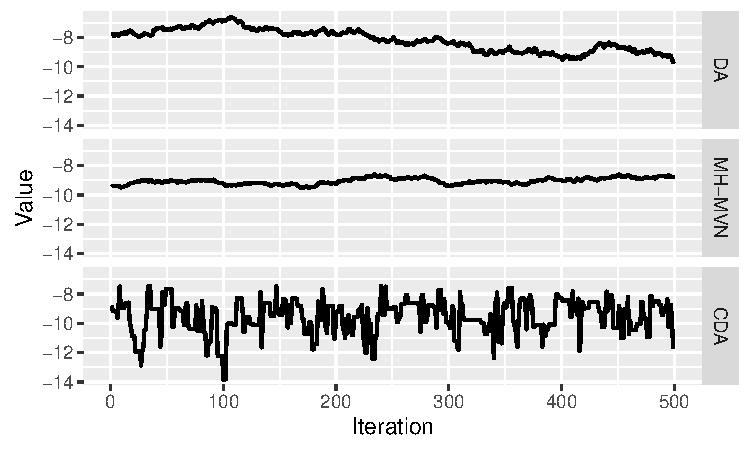
\includegraphics[width=1\textwidth]{logit_demo_trace_plot}
  \caption{Traceplots for DA, CDA and M-H with multivariate normal proposal.}
\end{subfigure}
  \hfill
   \begin{subfigure}[b]{0.49\textwidth}
 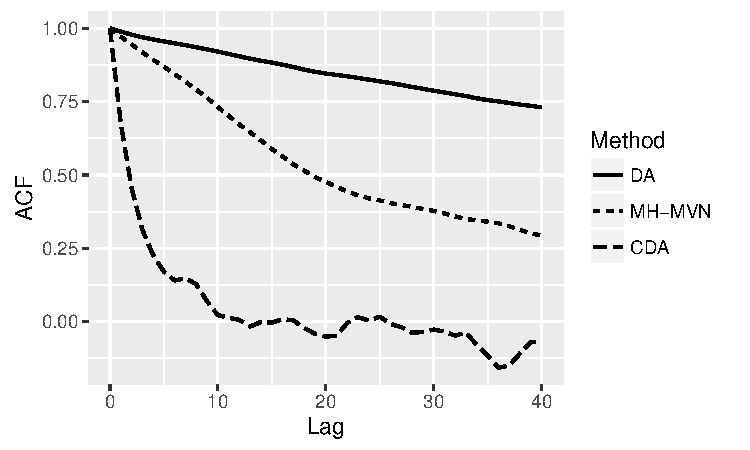
\includegraphics[width=1\textwidth]{logit_demo_acf}
  \caption{ACF for DA, CDA and M-H with multivariate normal proposal.}
\end{subfigure}
 \caption{Panel (a) demonstrates in traceplot and panel (b) in autocorrelation the substantial improvement of CDA in logistic regression with rare event data, compared with the original DA \citep{polson2013bayesian} and the M-H algorithm with multivariate normal proposal (MH-MVN).}
    \label{logit_random_mixing}
 \end{figure}




\section{Theory}

In this section, we provide theoretical support for CDA algorithms. Consider a Markov kernel $K((\theta,z);\cdot)$ with invariant measure $\Pi$ and update rule of the form \eqref{eq:da}, and a Markov chain $(\theta_t,z_t)$ on a state space $\Theta \times \mc Z$ evolving according to $K$. We will abuse notation in writing $\Pi(d\theta) = \int_{z \in \mc Z} \Pi(d\theta,dz)$. The lag-1 autocorrelation for a function $g : \Theta \to \bb R$ at stationarity can be expressed as the Bayesian fraction of missing information \citep{papaspiliopoulos2007general}
\be
\gamma_g &= 1- \frac{\bb E[\var(g(\theta) \mid z)]}{\var(g(\theta))}, \label{eq:missinginfo}
\ee
where the integrals in the numerator are with respect to $\Pi(d\theta,dz)$ and in the denominator with respect to $\Pi(d\theta)$. Let 
\be
L_2(\Pi) = \left\{ g : \Theta \to \bb R, \int_{\theta \in \Theta} \{g(\theta)\}^2 \Pi(d\theta) < \infty \right\} 
\ee
be the set of real-valued, $\Pi$ square-integrable functions. The \emph{maximal autocorrelation}
\be
\gamma = \sup_{g \in L^2(\Pi)} \gamma_g = 1- \inf_{g \in L^2(\Pi)} \frac{\bb E[\var(g(\theta) \mid z)]}{\var(g(\theta))}
\ee
is equal to the geometric convergence rate of the data augmentation Gibbs sampler \citep{liu2008monte}. For $g(\theta) = \theta_j$ a coordinate projection, the numerator of the last term of \eqref{eq:missinginfo} is, informally, the average squared step size for augmentation algorithm at stationarity in direction $j$, while the denominator is the squared width of the bulk of the posterior in direction $j$. Consequently, $\gamma$ will be close to 1 whenever the average step size at stationarity is small relative to the width of the bulk of the posterior, leading to slow mixing.

The purpose of CDA is to introduce working parameters that allow us to control the step size -- roughly speaking, the numerator of \eqref{eq:missinginfo} -- with greater flexibility than reparametrization or parameter expansion. The flexibility gains are achieved by allowing the invariant measure to change as a result of the introduced parameters. The working parameters $(r,b)$ correspond to a collection of reparametrizations, each of which defines a proper (but distinct) likelihood $L_{r,b}(\theta;y)$, and for which there exists an update rule of the form \eqref{eq:da}. Without using M-H step, one can derive a Gibbs sampler associated with $\theta$-marginal invariant measure $\Pi_{r,b}(\theta;y) \propto L_{r,b}(\theta;y) \Pi^0(\theta)$. We refer this sampler as calibrated Gibbs (C-Gibbs). But ultimately, we are interested in the original $\Pi(\theta;y)$, so we use one iteration of C-Gibbs as an efficient proposal for Metropolis-Hastings. That is, we propose $\theta^*$ from $Q(\theta;\cdot)$ where
\be \label{eq:Q}
Q_{r,b}(\theta;A) = \int_{(\theta^*,z) \in A \times \mc Z} \pi_{r,b}(z;\theta,y) f_{r,b}(\theta^*;z,y) dz d\theta^*
\ee
for $A \subseteq \Theta$, where $\pi_{r,b}$ and $f_{r,b}$ denote the conditional densities of $z$ and $\theta$ in C-Gibbs sampler with invariant measure $\Pi_{r,b}$. Similarly, we denote the Markov kernel as $K_{r,b}((\theta,z);(\theta^*,z'))$ for the transition from $(\theta,z)$ to $(\theta^*,z')$. By tuning working parameters during an adaptation phase to minimize the lag-1 autocorrelation for the identity function while optimizing the Metropolis-Hastings acceptance rate, we can select values of the working parameters that yield a computationally efficient algorithm.

 First, we show that CDA is ergodic. This is basically a consequence of C-Gibbs being ergodic for fixed $r,b$ and the fact that $\Pi_{r,b}$ and $\Pi$ are absolutely continuous with respect to Lebesgue measure on $\bb R^p$.
\begin{remark}[ergodicity]
Assume that $\Pi(d\theta)$ and $\Pi_{r,b}(d\theta)$ have densities with respect to Lebesgue measure on $\bb R^p$, and that $K_{r,b}((\theta,z);(\theta^*,z'))>0 \,\forall\, ((\theta,z),(\theta^*,z')) \in (\Theta \times \mc Z) \times (\Theta \times \mc Z)$. Then, for fixed $r,b$, C-Gibbs is ergodic with invariant measure $\Pi_{r,b}(d\theta,dz)$. Moreover, CDA, a Metropolis-Hastings algorithm with proposal kernel $Q_{r,b}(\theta^*;\theta)$ as defined in \eqref{eq:Q} with fixed $r,b$, is ergodic with invariant measure $\Pi(d\theta)$.
\end{remark}
\begin{proof}
For any $r,b$, the conditionals $\Pi_{r,b}(z \mid \theta)$ and $\Pi_{r,b}(\theta \mid z)$ are well-defined for all $z \in \mc Z, \theta \in \Theta$, and therefore the Gibbs transition kernel $K_{r,b}((\theta,z);\cdot)$ and corresponding marginal kernels $Q_{r,b}(\theta;\cdot)$ are well-defined. Moreover, for any $(z,\theta) \in \mc Z \times \Theta$, we have $\bb P[(\theta^*,z') \in A \mid (\theta,z)] > 0$ by assumption. Thus $K_{r,b}$ is aperiodic and $\Pi_{r,b}$-irreducible.

$Q_{r,b}(\theta^*;\theta)$ is aperiodic and $\Pi_{r,b}(\theta)$-irreducible, since it is the $\theta$ marginal transition kernel induced by $K_{r,b}((\theta,z);\cdot)$. Thus, it is also $\Pi(\theta)$-irreducible so long as $\Pi \gg \Pi_{r,b}$, where for two measure $\mu,\nu$, $\mu \gg \nu$ indicates absolute continuity. Since $\Pi, \Pi_{r,b}$ have densities with respect to Lebesgue measure, $\Pi_{r,b}$-irreducibility implies $\Pi$ irreducibility. Moreover, $Q(\theta;\theta^*) > 0$ for all $\theta \in \Theta$. Thus, by Theorem 3 of \cite{roberts1994simple}, CDA is $\Pi$-irreducible and aperiodic. 
\end{proof}

Having established ergodicity of both C-Gibbs and CDA under weak assumptions that hold for all of the data augmentation strategies we consider here, we now provide a semi-rigorous argument for why our approach to tuning $r$ and $b$ results in both rapid convergence and closeness of $\Pi_{r,b}$ to $\Pi$. Suppose there exists $r$ such that
\be
\bb E_{\Pi_{r,b}}[\var(\theta \mid z)] = \var_{\Pi}(\theta)
\ee
for any value of $b$. This is a simplification, since our adaptation strategies only allow us to control the discrepancy between the approximate marginal and expected conditional variance at certain fixed state.
By tuning $r$ during the adaptation phase, we make the lag-1 autocorrelation for the identity function small. 

This is obviously much weaker than minimizing the autocorrelation for worst-case functions. However, for the sake of exposition, we will proceed on the assumption that we can make the lag-1 autocorrelation for the identity function close to zero by appropriately tuning $r$. This makes the rationale for tuning $b$ to increase the Metropolis acceptance probability much clearer. First, we note the form of the Metropolis acceptance ratios, which we have used previously without rigorous justification.
\begin{remark}
The CDA acceptance ratio is given by
\be
\frac{L(\theta^*;y) \Pi^0(\theta^*) Q_{r,b}(\theta;\theta^*)}{L(\theta;y) \Pi^0(\theta) Q_{r,b}(\theta^*;\theta)} = \frac{L(\theta^*;y)L_{r,b}(\theta;y)}{L(\theta;y) L_{r,b}(\theta^*;y)} \label{eq:mh-accrat}
\ee
\end{remark}
\begin{proof}
Since $Q_{r,b}(\theta;\theta^*)$ is the $\theta$ marginal of a Gibbs transition kernel, and Gibbs is reversible on its margins, we have
\be
Q(\theta;\theta^*) \Pi_{r,b}(\theta) = Q(\theta^*;\theta) \Pi_{r,b}(\theta),
\ee 
and so
\be
\frac{L(\theta^*;y) \Pi^0(\theta^*) Q(\theta;\theta^*)}{L(\theta;y) \Pi^0(\theta) Q(\theta^*;\theta)} &= \frac{L(\theta^*;y) \Pi^0(\theta^*) L_{r,b}(\theta;y) \Pi^0(\theta) }{L(\theta;y) \Pi^0(\theta) L_{r,b}(\theta^*;y) \Pi^0(\theta^*)} \\
&= \frac{L(\theta^*;y)L_{r,b}(\theta;y)}{L(\theta;y) L_{r,b}(\theta^*;y)}.
\ee
\end{proof}

The expression in \eqref{eq:mh-accrat} will be near 1 at stationarity if 
\be 
\int \log \left( \frac{L(\theta^*;y)L_{r,b}(\theta;y)}{L(\theta;y) L_{r,b}(\theta^*;y)} \right) Q_{r,b}(\theta^*;\theta) \Pi(d\theta) \approx 0.
\ee
Now, suppose that a Markov chain evolving according to $K_{r,b}$ is rapidly mixing, so that for starting measures satisfying a condition like
\be
\sup_A \frac{\nu(A)}{\Pi_{r,b}(A)} < M
\ee 
for $M$ not too large we have 
\be
\KL{\Pi_{r,b}}{\int Q_{r,b}(\theta^*;\theta) \nu(d\theta)} \quad \textnormal{small}.
\ee
Then the symmetric KL is 
\be
\KL{\Pi_{r,b}}{\Pi} + \KL{\Pi}{\Pi_{r,b}} &= \int \Pi_{r,b}(d\theta) \log \frac{\Pi_{r,b}(\theta)}{\Pi(\theta)} + \int \Pi(d\theta) \log \frac{\Pi(\theta)}{\Pi_{r,b}(\theta)} \\
&= \int \Pi_{r,b}(d\theta) \log \frac{c_{r,b} L_{r,b}(\theta) \Pi_0(\theta)}{c L(\theta) \Pi_0(\theta)} + \int \Pi(d\theta) \log \frac{c L(\theta) \Pi_0(\theta)}{c_{r,b} L_{r,b}(\theta) \Pi_0(\theta)} \\
&\approx \int K_{r,b}(\theta^*;\theta) \Pi(d\theta) \log \frac{L_{r,b}(\theta^*)}{L(\theta^*)} + \int \Pi(d\theta) \log \frac{L(\theta)}{L_{r,b}(\theta)} \\
&= \bb E \left[ \frac{L_{r,b}(\theta^*) L(\theta)}{L_{r,b}(\theta) L(\theta^*)} \right],
\ee
for $\theta \sim \Pi$ and $\theta^* \mid \theta \sim K_{r,b}(\theta^*;\theta)$, so that tuning $b$ to make the M-H acceptance ratio larger will tend to make the symmetric KL between $\Pi_{r,b}$ and $\Pi$ small. As the acceptance ratio approaches 1, CDA and C-Gibbs coincide, and the C-Gibbs invariant measure is identically $\Pi$, but the corresponding sampler converges rapidly.

\section{Co-Browsing Behavior Application}

We now apply CDA to an online browsing activity dataset, in order to illustrate the application of CDA under more complicated setting such as hierarchical model and random effects. The dataset contains a two-way table of visit count, made by internet users who browsed one of $96$ client websites, and one of the  $n=59,792$ high-traffic sites during the same browsing session. We refer to the behavior of visiting more than one sites at the same session as ``co-browsing''. For each client site, it is of high commercial interests to identify the top few high-traffic sites with high co-browsing rates, in order to place more ads on those sites. For advertising company, it is useful to predict the traffic patterns between the high-traffic sites and their clients, so that the data collection can be less frequent on those clients that can be well predicted. We consider two models for these data.


\subsection{Hierarchical Binomial Model for Estimating Co-browsing Rates}

We first focus on one client website and analyze its co-browsing rates with the high-traffic sites. With the total visit count $N_i$ available for the $i$th high-traffic site, the count of co-browsing visit $y_i$ with the client of interests can be considered as the result of a binomial trial. With $y_i$ extremely small relative to $N_i$ (with ratio  ($0.00011 \pm  0.00093$)), the maximum likelihood estimate $y_i/N_i$ can have poor performance. For example, when $y_i=0$, estimating the rate as exactly $0$ is not ideal. Instead, it is useful to consider a hierarchical model that allows borrowing of information across high-traffic sites.

\be
 y_i & \sim \Binom\left(N_i, p_i\right),\quad p_i = \frac{\exp(\theta_i)}{1+\exp(\theta_i)}, \quad \theta_i\stackrel{iid}{\sim} \No(\theta_0, \sigma^2_0) \quad  i=1\ldots n\\
 (\theta_0,\sigma^2_0) & \sim  \pi(\theta_0,\sigma^2_0) 
\ee
Based on expert opinion in quantitative advertising, we use a weakly informative prior $\theta_0\sim \No(-12,49)$ and non-informative uniform prior on $\sigma^2_0$. 


Since $\theta_i \mid \theta_0, \sigma_0^2, y_i $ are conditionally independent, each $\theta_i$ can be sampled via CDA separately. For $i=1,\ldots,n$, we calibrate the binomial Polya-Gamma augmentation, leading to proposing from:

\be
z_i \mid  \theta_i, N_i &\sim \PG\left ( N_ir_i,\theta_i+b_i \right)\\
\theta_i^* \mid z_i, y_i, N_i &\sim \No \left( \frac{ y_i - r_i N_i/2 -z_i b_i + \theta_0/\sigma^2_0}{z_i+ 1/\sigma^2_0}, \frac{1}{z_i+ 1/\sigma^2_0}\right),
\ee
and accepting with probability
\be
1 \wedge  \frac{   L_{r,b}(\theta_i;y_i, N_i) L(\theta_i^*;y_i, N_i)}{  L_{r,b}(\theta_i^*;y_i, N_i)L(\theta_i;y_i,N_i) },
\ee
where 
\be
L_{r,b}(\theta_i;y_i, N_i) = \frac{\exp(\theta_i+b_i)^y_i}{\{ 1+\exp(\theta_i+b_i)\}^{N_ir_i}}
\ee
and $L(\theta_i;y_i, N_i) = L_{1,0}(\theta_i;y_i, N_i)$.  We require $r_i \in (0,1]$ to obtain increased or unchanged step size and $r_i > (y_i-1)/N_i$ to have a proper $L_{r,b}(\theta_i;y_i, N_i)$.

For adaptation of parameters in CDA, we use the empirical MAP  $\hat\theta_i$ based on each $L(\theta_i; y_i, N_i)\pi(\theta_i)$ to minimize $\Delta_{\mc I}(\hat\theta_i) $. We set $r_i = ( \hat r_i \vee ((y_i-1)/N_i + \epsilon)) \wedge 1$ with $\hat r_i = \frac{1}{c_0}\frac{\exp(\hat\theta_i)}{ \{1+\exp(\hat\theta_i)\} ^2} / \left (   \frac{1}{2 | \hat\theta_i+b_i|} \tanh\frac{|\hat\theta_i+b_i|}{2} \right)$ and $b_i=\log[  \{1+\exp(\hat\theta_i)\}^{1/r_i} -1] - \hat\theta_i$, with $ \epsilon$ as small positive number to ensure $L_{r,b}(\theta_i;y_i, N_i)$ is proper. The default $c_0=1$ leads to a high average acceptance of $0.9$ for all $\theta_i$.

After $\theta_i$'s are updated, other parameters are sampled from $\theta_0 \sim \No\big( (n/\sigma^2 +1/49)^{-1} (\sum_i \theta_i /\sigma^2  -12/49 ),  (n /\sigma^2 +1/49)^{-1} \big)$ and $\sigma^2_0 \sim \IG( n/2-1, \sum_i (\theta_i -\theta_0)^2 /2)$.

Figure~\ref{data_binomial} shows the boxplots of the ACFs for all $\theta_i$'s. We compare the result with the original DA \citep{polson2013bayesian} and Hamiltonian Monte Carlo (HMC) provided by the \texttt{STAN} software \citep{carpenter2016stan}. We run DA for $100,000$ steps, HMC for $2000$ steps and CDA for $2,000$ steps, so that they have approximately the same effective sample size (calculated with the \texttt{CODA} package in \texttt{R}). All of the parameters mix poorly in DA; HMC and CDA leads to significant improvement with autocorrelation rapidly decaying to close to zero within $5$ lags.

Shown in Table~\ref{tab:binomial}, CDA and HMC have very close estimates in posterior means and $95\%$ credible intervals for the parameters; while DA has poor estimates due to critically slow mixing. The difference between HMC and CDA is that, although HMC is slightly more efficient in effective sample size per iteration ($T_{eff}/T$) for this model, it is much more computationally intensive and generate much less iterations than CDA, within a same budget of computing time. As the result, CDA has the most efficient computing time per effective sample.
 


 \begin{figure}[H]
 % \centering
   \begin{subfigure}[b]{0.32\textwidth}
 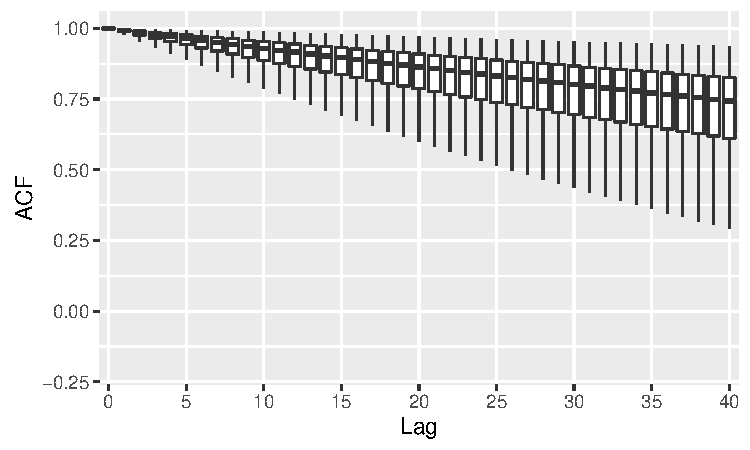
\includegraphics[width=1\textwidth]{binomial_random_acf_da.pdf}
 \caption{ACFs of the rate parameters $\theta_i$ using DA.}
 \end{subfigure}
  \hfill 
 \begin{subfigure}[b]{0.32\textwidth}
 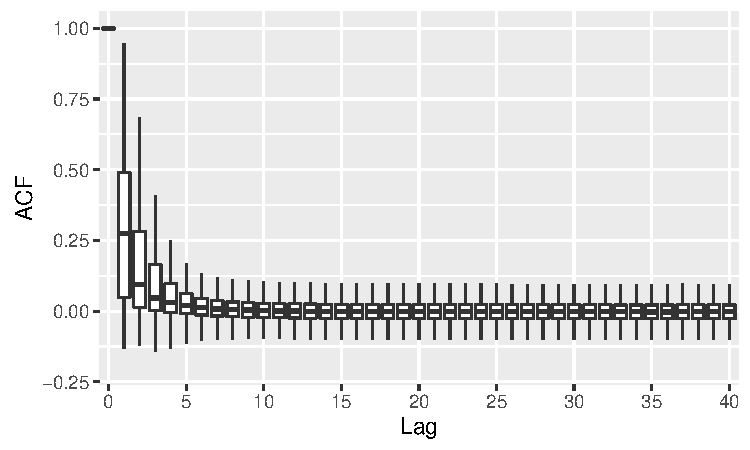
\includegraphics[width=1\textwidth]{binomial_random_acf_cda.pdf}
 \caption{ACFs of the rate parameters $\theta_i$ using CDA.}
 \end{subfigure} 
   \hfill 
 \begin{subfigure}[b]{0.32\textwidth}
 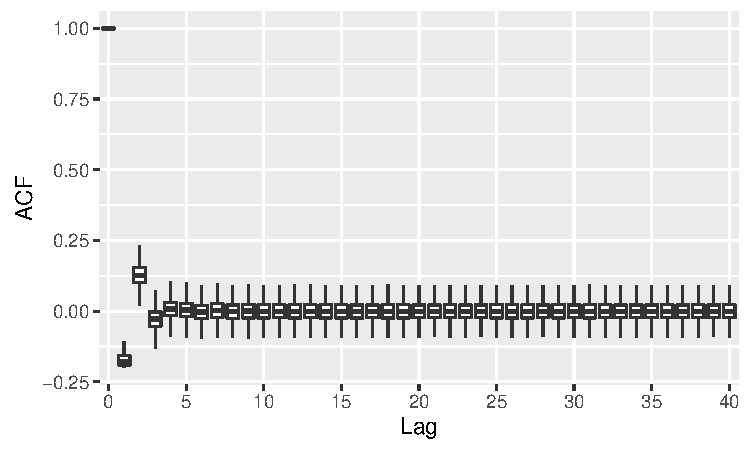
\includegraphics[width=1\textwidth]{binomial_random_acf_hmc.pdf}
 \caption{ACFs of the rate parameters $\theta_i$ using HMC.}
 \end{subfigure} 
 \caption{Boxplots of the ACFs show the mixing of the $59,792$ parameters in the hierarchical binomial model, for the original DA\citep{polson2013bayesian}, CDA and HMC.}
 \label{data_binomial}
 \end{figure}
 
 
 
\begin{table}[H]
\centering
\begin{tabular}{|l |r |r| r| r |} 
 \hline
                          & DA & CDA & HMC\\
 [0.5ex]

 $ \sum \theta_i/n$      & -10.03 (-10.16, -9.87)& -12.05 (-12.09, -12.02) &  -12.06 (-12.09, -12.01)\\
 $ \sum \theta_i^2/n$      & 102.25 (98.92, 105.23)& 153.04 (152.06, 154.05) &  153.17 (152.02, 154.29)\\
$\theta_0$          & -10.03 (-10.17, -9.87)& -12.05 (-12.09,-12.01) &  -12.06 (-12.10, -12.01)\\
$\sigma^2$         & 1.60 (1.36, 1.82)&   7.70 (7.49, 7.88)  & 7.71 (7.51, 7.91)\\
$T_{eff} / T$ & 0.0085 (0.0013 0.0188) & 0.5013 (0.1101,1.0084) & 0.8404 (0.5149, 1.2470)\\
Computing Time /  $T$  & 1.2 sec       & 1.2 sec        & 6 sec\\
Computing Time /  $T_{eff}$  & 140.4 sec       & 0.48 sec        & 1.3 sec\\
 \hline
\end{tabular}
\caption{Parameter estimates (with 95\% credible intervals) and computing speed (ratios among computing time, effective sample sizes $T_{eff}$ and total iterations $T$) of the DA, CDA and HMC in hierarchical binomial model. CDA provides parameter estimates as accurate as HMC, and is more computationally efficient than HMC.}
\label{tab:binomial}
\end{table}


\subsection{Poisson Log-Normal Model for Web Traffic Prediction}

As a second application, since one co-browsing record of each high-traffic and client pair sites usually indicates a link for user to click through to go from one to another, the total count of co-browsing can be treated as a surrogate for click-through traffic. For the advertising company with historic data, comparing the co-browsing records clients can reveal the predictive patterns among clients, hence reduce the frequency of tracking those clients that can be well predicted.

We consider a Poisson regression model. For illustration, we choose the co-browsing count of one client website as the outcome $y_i$, and the count of other $95$ websites as the covariates $w_{i,j}$ for $i=1\ldots n$ with $n=59,792$ and $j=1\ldots p$ with $p=95$. To use them as predictors in Poisson log-normal model, we transform the count onto the log scale with $x_{i,j}=\log (w_{i,j}+1)$. We use a normal random intercept $\tau_i$ for each $i$ to allow over-dispersion. We the random intercepts have a common mean $\tau_0$, so that we do not need a fixed effect intercept.

\be
 y_i \sim \Poi \left( \exp  (\xbeta + \tau_i )\right),  \quad \tau_i\stackrel{iid}{\sim} \No(\tau_0, \nu^2) \quad i=1\ldots n\\
 \beta \sim  \No(0, I \sigma_\beta^2), \quad \tau_0 \sim \No(0,\sigma_\tau^2) \quad \nu^2\sim \pi(\nu^2),
\ee
where $\xbeta= \sum_j x_{i,j}\beta_j$. We assign a diffuse prior for $\beta$ and $\tau_0$ with $ \sigma_\beta^2=\sigma_\tau^2=100$. For the over-dispersion parameter $\nu^2$, we assign a non-informative uniform prior.

We first exclude other factors that could contribute to slow mixing. In this case, when $\beta$ and $\tau$ are sampled separately, the random effects $\tau = \{\tau_1,\ldots, \tau_n\}$ can cause slow mixing. Instead, we sample $\beta$ and $\tau$ jointly. Using $\tilde X = [ I_n || X ]$ as a $n \times (n+p)$ juxtaposed matrix, and $\eta_i=\xbeta + \tau_i$ for the linear predictor, the model can be viewed as a linear predictor with $n+p$ coefficients, and $\theta= \{\tau, \beta\}'$ can be sampled jointly in a block. The reason for improved mixing with blocked sampling can be found in \cite{liu1994collapsed}.

We now focus on the mixing behavior due to data augmentation. We first review the the data augmentation for Poisson log-normal model. \cite{zhou2012lognormal} proposed to treat $\Poi(\eta_i)$ as the limit of the negative binomial $\NB(\lambda,\frac{\eta_i}{\lambda+\eta_i})$ with $\lambda\rightarrow \infty$, and used moderate $\lambda=1,000$ for approximation. The limit can be simplified as (omitting constant):

\be
L(\eta_i;y_i)=\frac{ \exp(y_i \eta_i \} }{\exp\{\exp(\eta_i)\}} = \lim_{\lambda\rightarrow\infty}\frac{\exp(y_i \eta_i)}{\{1+ \exp(\eta_i )/\lambda\}^{\lambda }}.
\label{eq:pos_approx}
\ee

With finite $\lambda$ approximation, the posterior can be sampled via Polya-Gamma augmented Gibbs sampling:

\be
z_i \mid \eta_i \sim  \PG ( & \lambda, \eta_i -\log \lambda)  \quad i=1\ldots n\\
\theta \mid z, y \sim  \No \big (  &  (\tilde X' Z \tilde X+  \begin{bmatrix} 1/\nu^2 \cdot I_n & 0\\ 0 & 1/\sigma^2_{\beta}  \cdot I_p \end{bmatrix})^{-1} \{  \tilde X'  \big ( y - \lambda/2 + Z \log \lambda\big) +   \begin{bmatrix} \tau_0/\nu^2  1_n \\  0_p \end{bmatrix} \} , \\
& (\tilde X' Z \tilde X+  \begin{bmatrix} 1/\nu^2 \cdot I_n & 0\\ 0 & 1/\sigma^2_{\beta}  \cdot I_p \end{bmatrix})^{-1} \big ),
\ee
where $Z = \diag\{ z_1, \ldots,  z_n\}$, $1_n = \{1, \ldots 1\}'$ and $0_p = \{0, \ldots 0\}'$.

Although this approximation enables closed-form posterior sampling, it is prone to cause slow mixing. To control approximation error, $\lambda$ needs to be large, but would generate large $Z$ and small conditional variance for $\theta \mid z, y$. In fact, for moderately large $\eta_i \approx 10$, $\lambda$ needs to be at least $10^9$ to make $\exp(2\eta_i)/\lambda$ close to $0$, as the expansion in \eqref{eq:pos_approx} has $(1+\exp\left(\eta_i)/\lambda\right)^\lambda= \exp \{ \exp(\eta_i) + \bigO(\exp(2\eta_i)/\lambda) \}$. This means a good control on approximation error would lead to an almost complete stop in the mixing.

We use CDA to solve this dilemma. We replace $\lambda$ with $r_i\lambda$, where $\lambda$ is set to $10^9$ and $r_i$ is a small fraction to allow calibration of the mixing behavior. With smaller $r_i\lambda$, we generate proposal that are much less correlated to the current state, then M-H step corrects the target to exact Poisson. Adding location adjusting parameter $b$, this leads to a proposal rule:

\be
z_i \sim  \PG ( & r_i\lambda, \eta_i -\log \lambda + b_i)  \quad i=1\ldots n\\
\theta^* \sim  \No \big(  &  (\tilde X' Z \tilde X+  \begin{bmatrix} 1/\nu^2 \cdot I_n & 0\\ 0 & 1/\sigma^2_{\beta}  \cdot I_p \end{bmatrix})^{-1} \{  \tilde X'  \big ( y - r\lambda/2 + Z \log (\lambda -b )\big) +   \begin{bmatrix} \tau_0/\nu^2  1_n \\  0_p \end{bmatrix} \} , \\
& (\tilde X' Z \tilde X+  \begin{bmatrix} 1/\nu^2 \cdot I_n & 0\\ 0 & 1/\sigma^2_{\beta}  \cdot I_p \end{bmatrix})^{-1} \big)
\ee
with acceptance probability
\be
1 \wedge  \prod_i \frac{   L_{r,b}(\eta_i ;y_i) L(\eta_i^*;y_i)}{  L_{r,b}(\eta_i^*;y_i)L(\eta_i;y_i) },
\ee
where 
\be
L_{r,b}(\eta_i;y_i) =\frac{\exp(y_i (\eta_i +b_i))}{\{1+ \exp(\eta_i+b_i )/r_i\lambda\}^{r_i\lambda }}, \quad L(\eta_i;y_i) =\frac{ \exp(y_i \eta_i \} }{\exp\{\exp(\eta_i)\}},
\ee
where $L(\theta_i;y_i)=L_{\infty,0}(\eta_i;y_i)$. To ensure increased or unchanged step size compared to basic algorithm where $r=1$, we require $r_i \in (0,1]$; to have proper $L_{r,b}(\eta_i;y_i)$, we need $r_i > (y_i-1)/\lambda$.

We use a tuning period to find the optimal values for calibration parameters. By minimizing $\Delta_{\mc I}(\hat\eta)$, we set $r_i = (\hat r_i  \vee ((y_i-1)/\lambda + \epsilon)) \wedge 1$ with $\hat r_i =1/c_0 \exp(\hat\eta_i) /  \left( \frac{\lambda } {2|\hat\eta_i + b_i - \log\lambda|}  \tanh\frac{ |\hat\eta_i + b_i - \log\lambda|}{2} \right )$ where $\hat\eta_i $ is the empirical MAP during tuning, $\epsilon$ is a small positive number to ensure $L_{r,b}(\eta_i;y_i)$ is proper. We found that the default  $c_0 =1$ resulted in the acceptance being too low. This indicates the inverse Fisher information based approach over-estimated the step size in this finite sample. We then use $c_0 = 0.1$ so that the amount of variance increase is reduced. This increased the acceptance rate to $0.6$. To reduce distance between $L_{r,b}(\eta_i;y_i)$ and $L(\eta_i;y_i)$, we used $b_i=\log[ \exp \{ \exp(\hat\eta_i - \log\lambda -\log r_i)   \}-1] -\hat\eta_i + \log\lambda$. After $\theta$ is updated, the other parameters can be sampled via $\tau_0\sim \No\left( (n/ \nu^2 + 1/ \sigma^2_\tau)^{-1} \sum_i \tau_i/\nu^2 , (n/ \nu^2 + 1/ \sigma^2_\tau)^{-1}  \right)$ and $\nu^2 \sim \IG ( n/2-1, \sum_i (\tau_i-\tau_0)^2 /2)$.

We ran the basic DA with $\lambda=1,000$ approximation, CDA with $\lambda=10^9$ and HMC. We ran DA for $200,000$ steps, CDA for $2,000$ steps and HMC for $20,000$ steps so that they have approximately the same effective sample size. For CDA, we used the first $1,000$ steps for adapting $r$ and $b$. Figure~\ref{data_poisson} shows the mixings of DA, CDA and HMC. Even with small $\lambda = 1,000$ in DA, all of the parameters mix poorly; HMC seemed to be affected by the presence of random effects, and most of parameters remain highly correlated within $40$ lags; CDA substantially improves the mixing. Table~\ref{table:Poisson} compares all three algorithms. CDA has the most efficient computing time per effective sample, and is about $30-300$ times more efficient than the other two algorithms.


 \begin{figure}[H]
 % \centering
  \begin{subfigure}[b]{0.32\textwidth}
 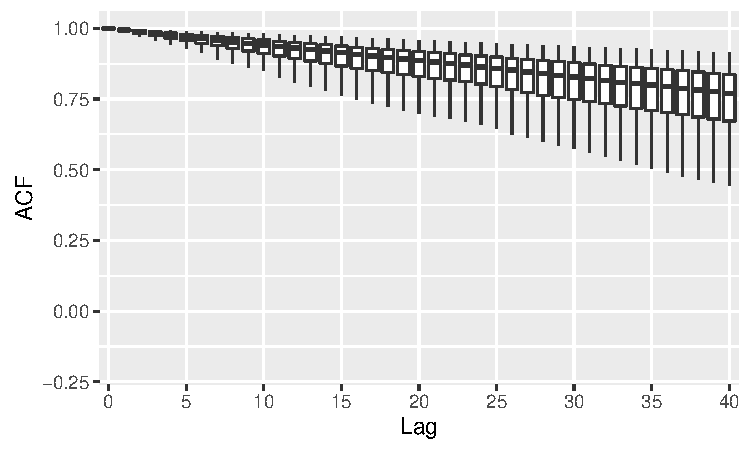
\includegraphics[width=1\textwidth]{poisson_acf_da}
 \caption{Autocorrelation of the parameters from DA.}
 \end{subfigure}
  \hfill 
 \begin{subfigure}[b]{0.32\textwidth}
 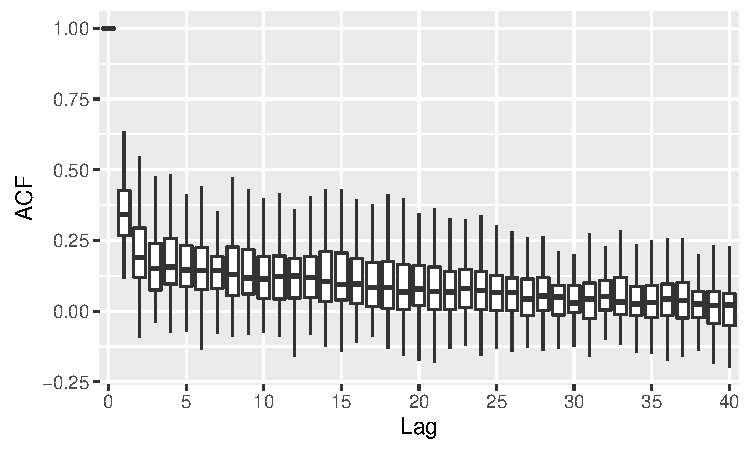
\includegraphics[width=1\textwidth]{poisson_acf_cda}
 \caption{Autocorrelation of the parameters from CDA.}
 \end{subfigure}  \hfill 
 \begin{subfigure}[b]{0.32\textwidth}
 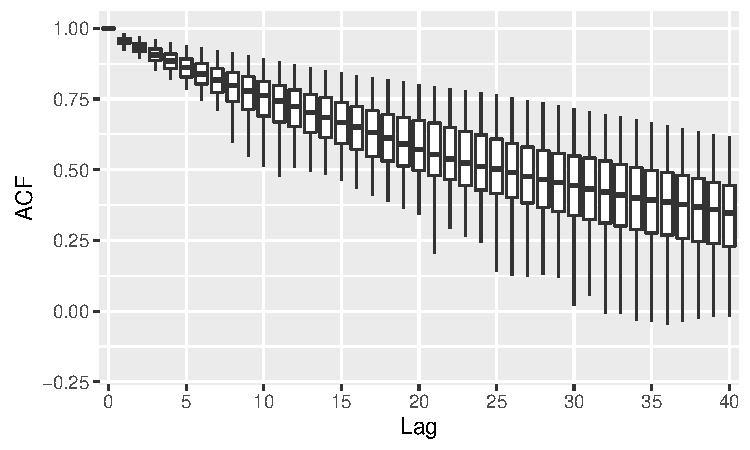
\includegraphics[width=1\textwidth]{poisson_acf_hmc}
 \caption{Autocorrelation of the parameters from HMC.}
 \end{subfigure}
 \caption{CDA significantly improves the mixing of the parameters in the Poisson log-normal.}
 \label{data_poisson}
 \end{figure}



To evaluate the prediction performance, we use another co-browsing count table for the same high traffic and client sites, collected during a different time period. We use the high traffic co-browsing count of $p= 95$ clients $ w_i^\dagger = \{  w_{i,1}^\dagger,  w_{i,2}^\dagger \ldots  w_{i,p}^\dagger \}$ with its log transform $  x^\dagger_{i} = \log(   w_{i}^\dagger +1 )$ to make prediction $\hat y_i^\dagger= \bb E_{ \beta, \tau \mid y,x}   y_{i}^\dagger =\bb E_{ \beta, \tau \mid y,x}\exp(  x_{i}^\dagger\beta + \tau_i)$ on the client site. The expectation is taken over posterior sample $\beta, \tau \mid y,x$ with training set $\{y,x\}$ discussed above. Cross-validation root-mean-squared error $\big(\sum_i(\hat y_i^\dagger - y_i^\dagger)^2/n\big)^{1/2}$ between the prediction and actual count $ y_i^\dagger$'s is computed. Shown in Table~\ref{table:Poisson}, slow mixing in DA and HMC cause poor estimation of the parameters and high prediction error, while CDA is significantly better. 


\begin{table}[H]
\centering
\begin{tabular}{|l |r |r| r| r |} 
 \hline
                          & DA & CDA & HMC\\
 [0.5ex]
$\sum \beta_j / 95$         & 0.072 (0.071, 0.075)&  -0.041 (-0.042, -0.038)  & -0.010 (-0.042, -0.037) \\
$\sum \beta_j^2 / 95$         & 0.0034 (0.0033, 0.0035)&  0.231 (0.219 0.244)  & 0.232 (0.216 0.244)   \\
$\sum\tau_i/n$         & -0.405 (-0.642, -0.155)&  -1.292 (-2.351, -0.446)  &  -1.297 (-2.354, -0.451)  \\
$\sum\tau_i^2/n$         & 1.126 (0.968, 1.339)&  3.608 (0.696, 7.928)  & 3.589 (0.678, 8.011)  \\
% RMSE                              & 30.83        & 4.03          & 7.38\\
Prediction RMSE                           & 33.21        & 8.52          & 13.18\\
$T_{eff} / T$ & 0.0037 (0.0011 0.0096) & 0.3348 (0.0279, 0.699) &  0.0173 (0.0065, 0.0655) \\
Computing Time /  $T$  & 1.3 sec       & 1.3 sec        & 56 sec\\
Computing Time /  $T_{eff}$  & 346.4 sec       & 11.5 sec        & 3240.6 sec\\
 \hline
\end{tabular}
\caption{Parameter estimates, prediction error and computing speed of the DA, CDA and HMC in Poisson regression model.}
\label{table:Poisson}
\end{table}

\section{Discussion}
Data augmentation is a technique routinely used to sample posterior in closed-form. Despite the convenience, it could slow down the mixing, as the step size becomes smaller than the marginal variance. At the age of ``big $n$'' data, any concentration rate difference between the two will lead to a near stop in posterior mixing as $n$ increases. To our best knowledge, although the previous methods such as centered or non-centered re-parameterization \citep{papaspiliopoulos2007general} and parameter-expansion \citep{liu1999parameter} lead to some improvement in small dataset, they do not fundamentally solve the rate difference problem in large data.

Our proposed CDA method directly tackles this issue by adjusting the step size to the same order of the unconditional variance. The generated samples are used as proposals in M-H step to obtain correct posterior. As the original un-calibrated Gibbs sampler is a special case of CDA with certain $r$ and $b$, CDA can be viewed as a generalized class of sampling algorithms with data augmentation. CDA adds a little cost during likelihood evaluation, but its burden is often negligible as dominated by other tasks, mostly random number generation. In this article, we demonstrate that calibration is generally applicable when the conditional $\theta \mid z$ given latent variable $z$ belongs to the location-scale family. We expect it to be extensible to any conditional distribution with a variance or scale.

As both CDA and HMC involve M-H step, we draw some further comparison between the two. Both methods rely on finding good proposal through searching over a region far from the current state. The key difference lies in the computing efficiency in generating proposal. To generate one proposal, HMC often requires multiple iterations in Hamiltonian dynamics, which are computationally intensive; in contrast, CDA only requires one iteration of sampling. Therefore, CDA is likely to be much more efficient than HMC. Although we discuss calibration in the context of data augmentation, the idea can be more generally applicable to most Gibbs sampling to adjust its step size for faster mixing. 

\bibliography{reference}
\bibliographystyle{plainnat}

%
%\section{Appendix}
%
%\subsection{Goodness-of-Fit and Cross-Validation for Poisson Regression}
%
%
% \begin{figure}[H]
% % \centering
%   \begin{subfigure}[b]{0.45\textwidth}
% 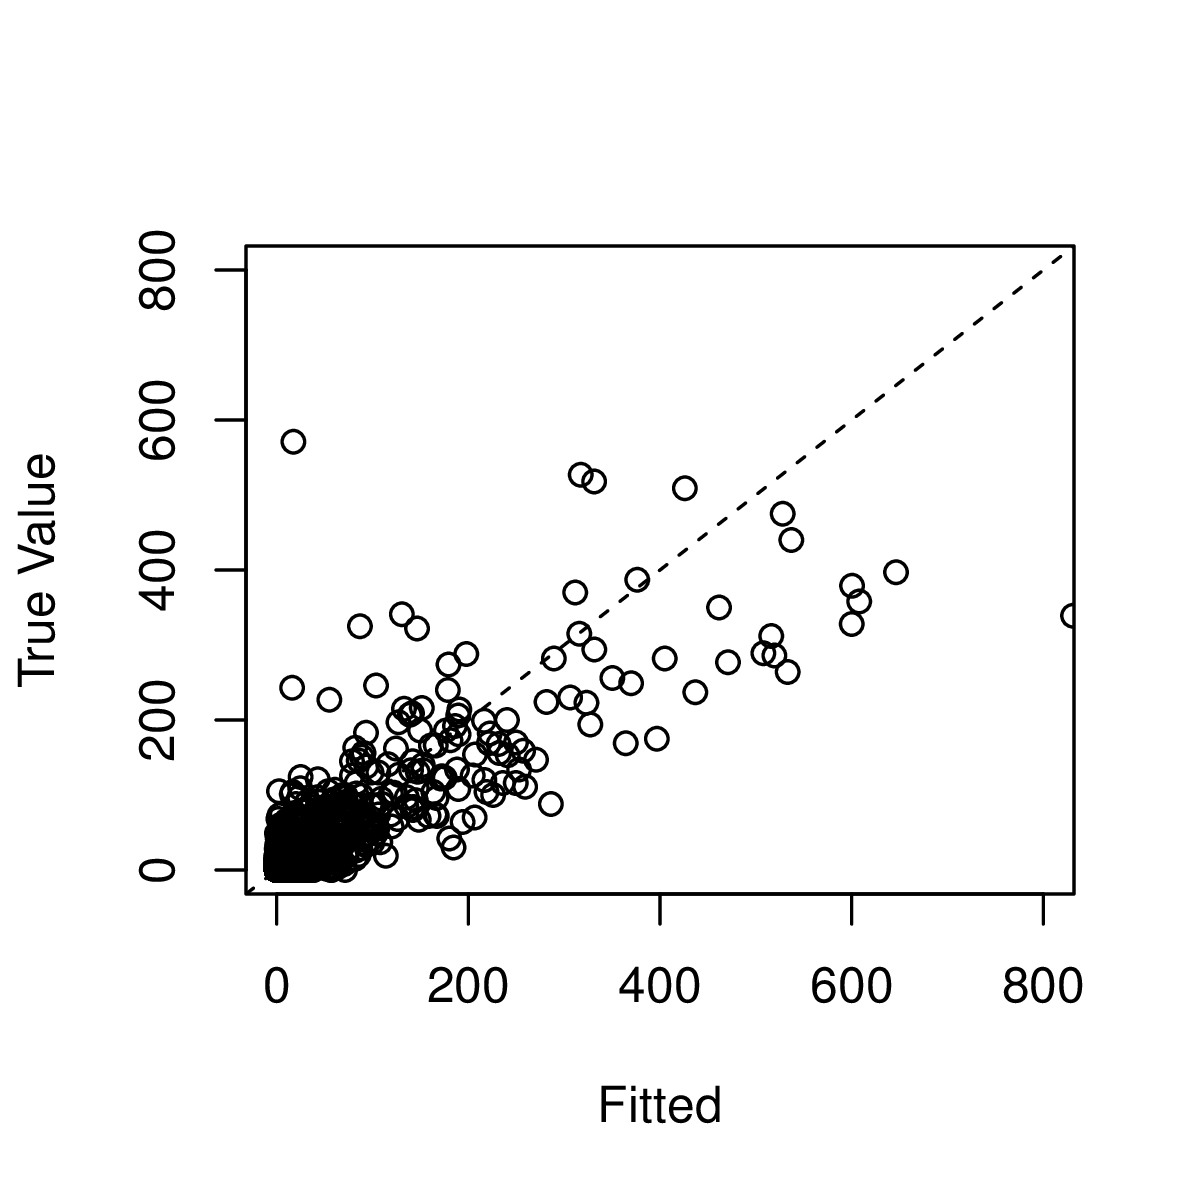
\includegraphics[width=1\textwidth]{poisson_fitting_da.png}
% \caption{Fitted vs true values using DA}
% \end{subfigure}
%  \hfill 
% \begin{subfigure}[b]{0.45\textwidth}
% 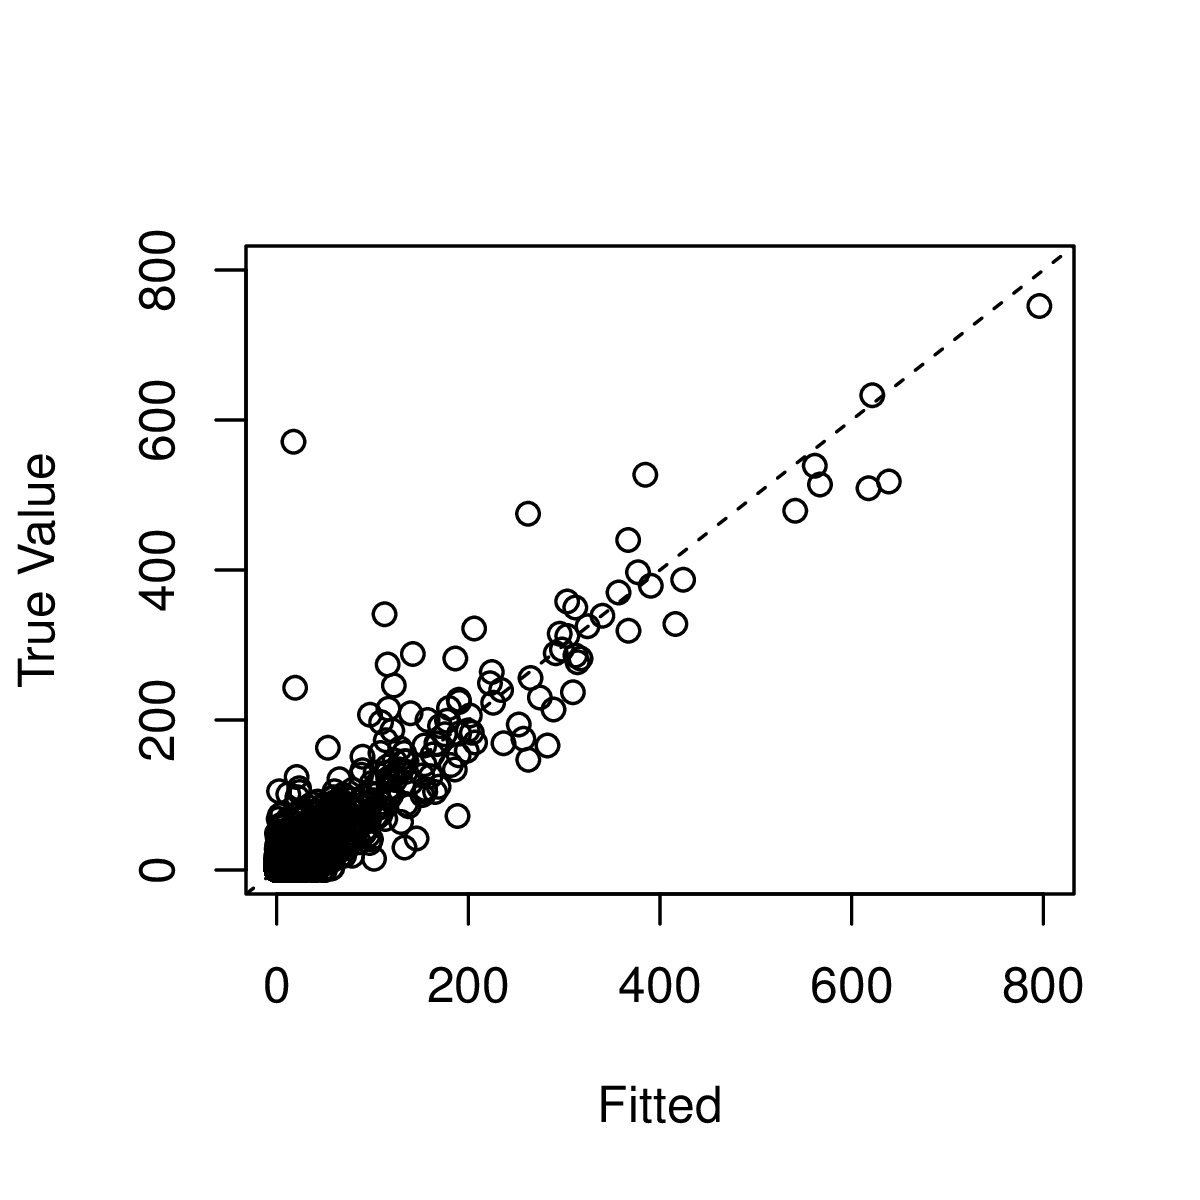
\includegraphics[width=1\textwidth]{poisson_fitting_ada.png}
% \caption{Fitted vs true values using CDA}
% \end{subfigure}  
%   \begin{subfigure}[b]{0.45\textwidth}
% 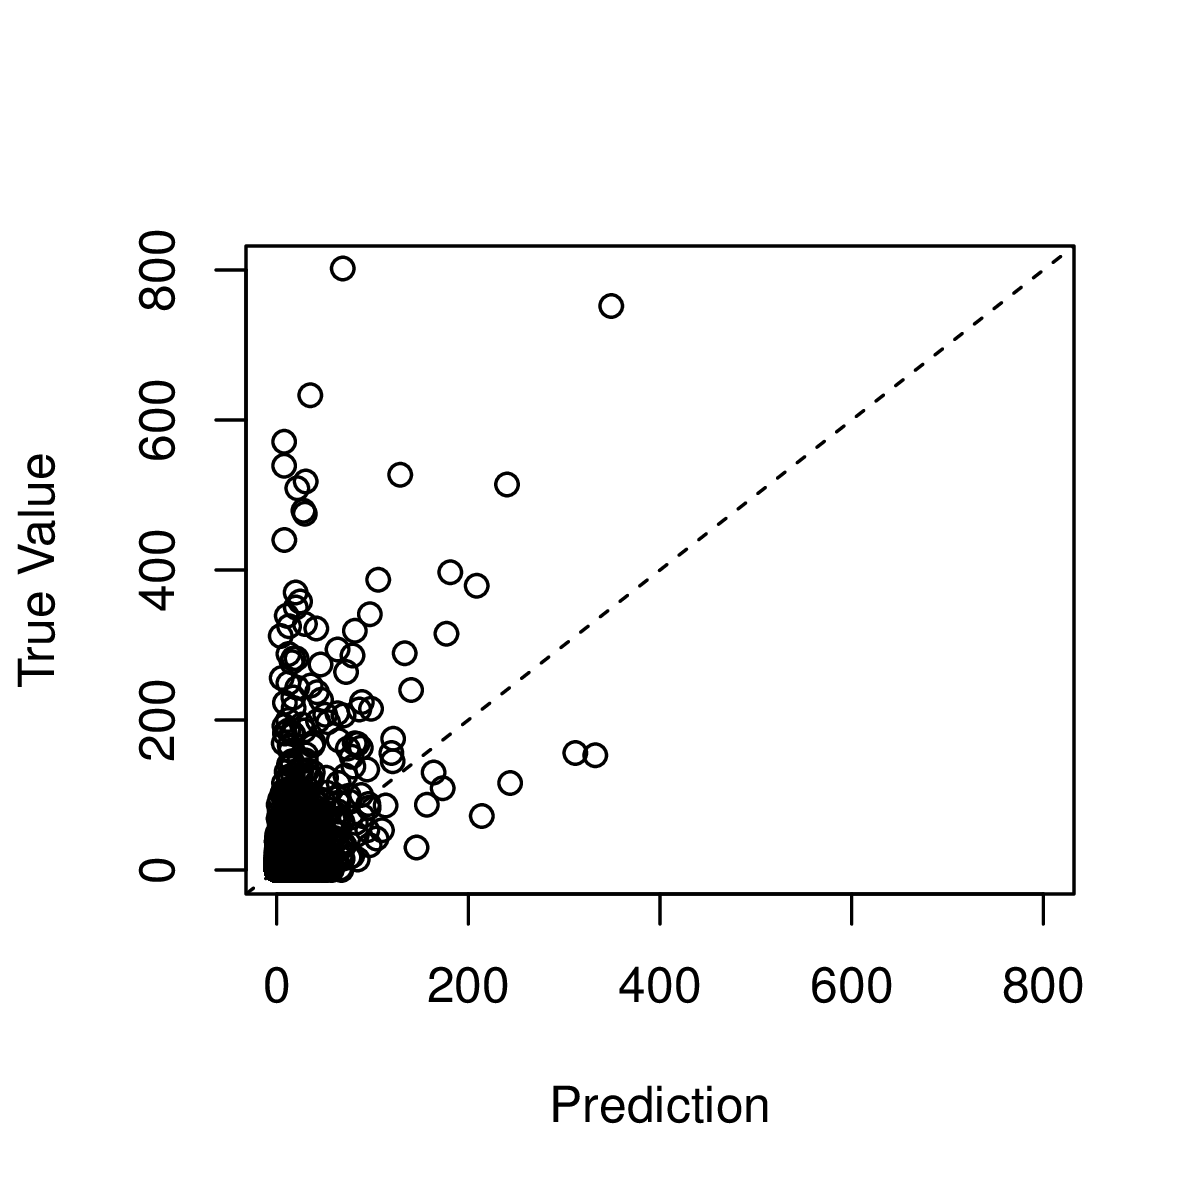
\includegraphics[width=1\textwidth]{poisson_cv_da.png}
% \caption{Prediction vs true values using DA}
% \end{subfigure}
%  \hfill 
% \begin{subfigure}[b]{0.45\textwidth}
% 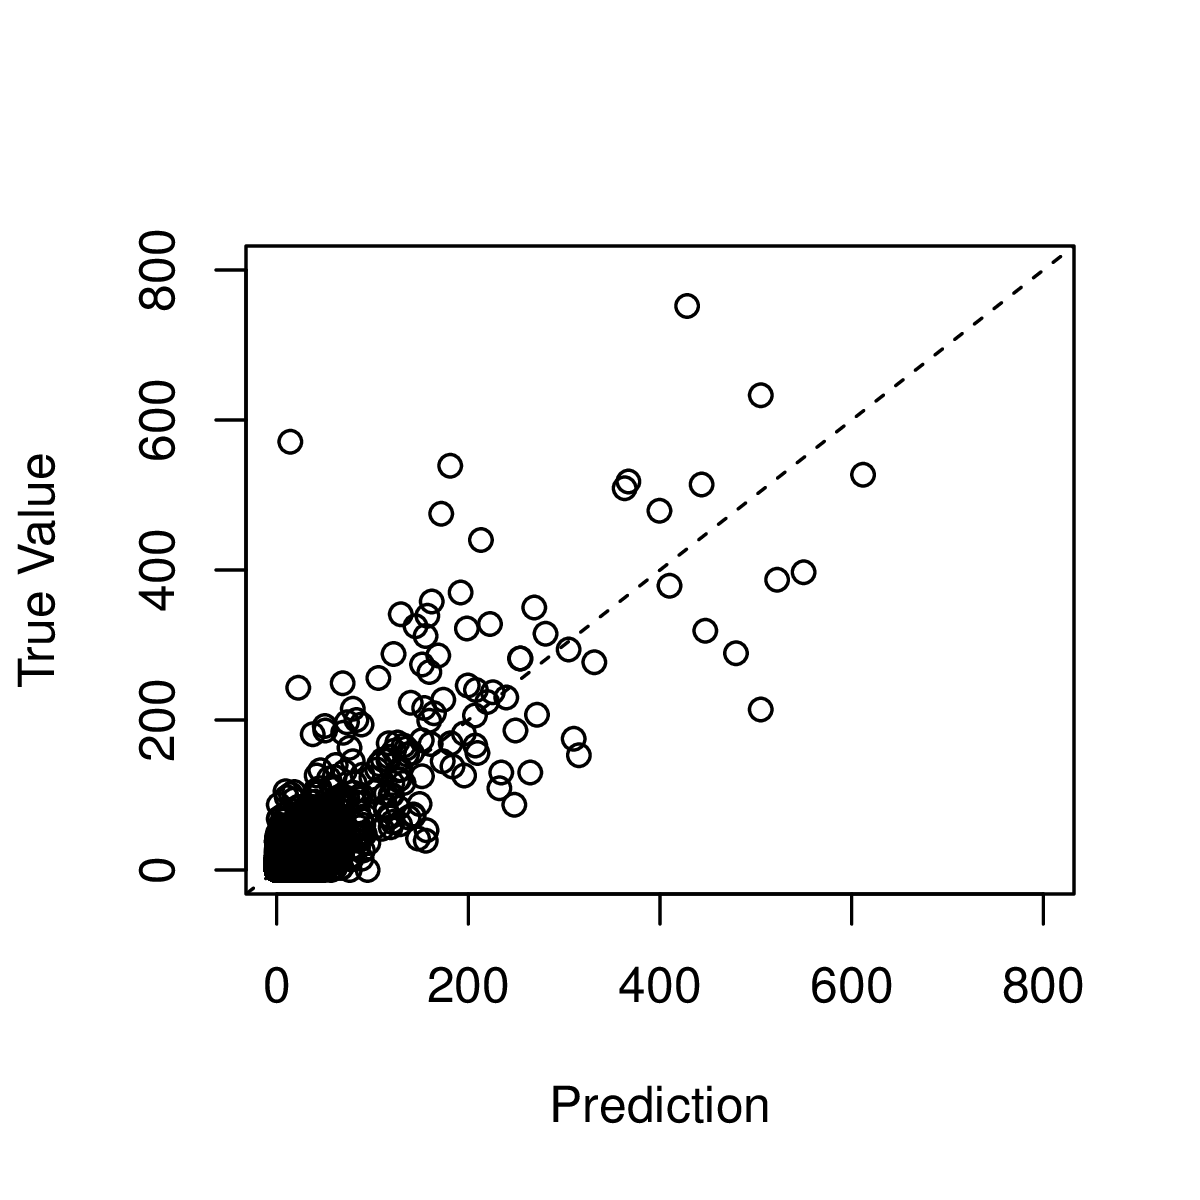
\includegraphics[width=1\textwidth]{poisson_cv_ada.png}
% \caption{Prediction vs true values using CDA}
% \end{subfigure} 
% \caption{The posterior estimates produced by CDA is better fitted to the data and have more accurate prediction than DA.}
% \end{figure}

 % \subsection{Comparing posterior samples of CDA with HMC}
% \begin{figure}[H]
%  % \centering
%    \begin{subfigure}[b]{0.45\textwidth}
%  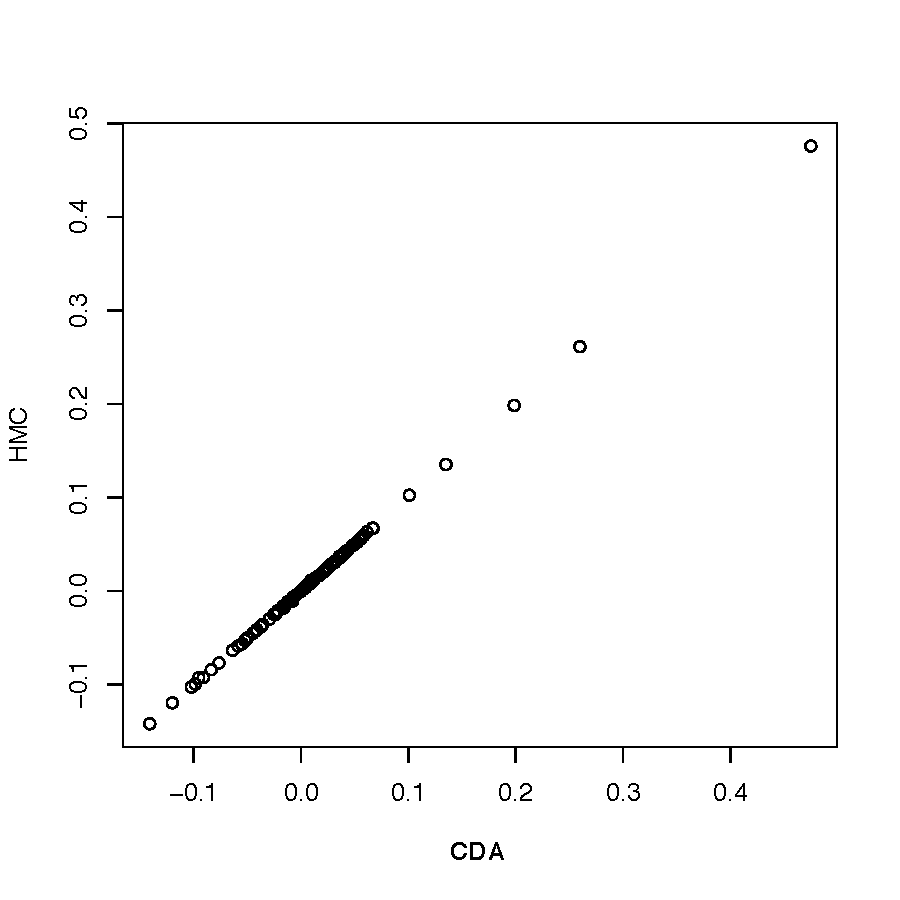
\includegraphics[width=1\textwidth]{CDAvsHMC_mean.pdf}
%  \caption{Comparing posterior means for $\theta_1,\dots \theta_{95}$ from the HMC and CDA. The  RMSE between the two is $0.0007$.}
%  \end{subfigure}
%   \hfill 
%  \begin{subfigure}[b]{0.45\textwidth}
%  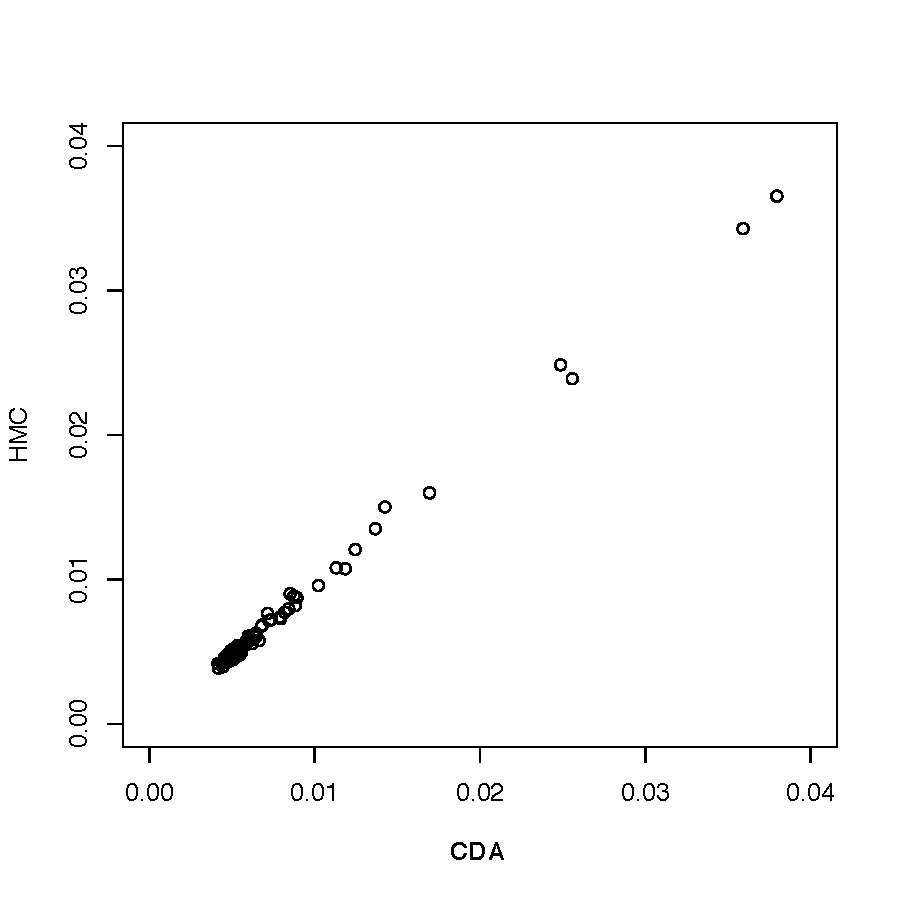
\includegraphics[width=1\textwidth]{CDAvsHMC_sd.pdf}
%  \caption{Comparing posterior standard deviation for $\theta_1,\dots \theta_{95}$ from the HMC and CDA.  The  RMSE between the two is $0.0004$.}
%  \end{subfigure}  
%  \caption{The results from CDA and HMC agree very well.}
%  \end{figure}





 
\end{document}




